\documentclass[conference,letterpaper,10pt]{IEEEtran}

\usepackage[T1]{fontenc}
\usepackage[utf8]{inputenc}
\usepackage[english,spanish,es-tabla,es-noshorthands,es-nodecimaldot]{babel}
\usepackage{microtype}
\usepackage{amsmath,amssymb}
\usepackage{graphicx}
\usepackage{booktabs,array,tabularx,multirow}
\usepackage{xcolor}
\usepackage{cite}
\usepackage{xurl}
\usepackage{balance}
\usepackage{placeins}
\setcounter{topnumber}{4}\setcounter{bottomnumber}{3}\setcounter{totalnumber}{6}\setcounter{dbltopnumber}{3}
\renewcommand{\topfraction}{0.96}\renewcommand{\bottomfraction}{0.80}\renewcommand{\textfraction}{0.03}
\renewcommand{\floatpagefraction}{0.85}\renewcommand{\dbltopfraction}{0.96}\renewcommand{\dblfloatpagefraction}{0.85}
\setlength{\textfloatsep}{8pt plus 2pt minus 3pt}\setlength{\dbltextfloatsep}{8pt plus 2pt minus 3pt}
\setlength{\floatsep}{7pt plus 2pt minus 2pt}\setlength{\dblfloatsep}{7pt plus 2pt minus 2pt}
\usepackage[hidelinks,pdftitle={BioBot-Rescue: red de mochilas embebidas en FPGA para localizar personas atrapadas},
  pdfauthor={Roberto Orozco Ramírez, Adam Del Pozo Ontiveros, Enrique Bernal Martín Prieto}]{hyperref}

\graphicspath{{../figs/}{../figs/rtl/}{../../layout/resultados/}{../images/}}
\definecolor{Primary}{HTML}{0E2A47}
\definecolor{Secondary}{HTML}{1D6FA5}
\newcommand{\Gp}{\textit{G.~portentosa}}
\newcommand{\sig}[1]{{\small\texttt{#1}}}
\newcommand{\tabfont}{\footnotesize}
\renewcommand{\arraystretch}{1.08}
\renewcommand{\IEEEkeywordsname}{Palabras clave}
\hyphenation{Li-bre-La-ne Goer-tzel CORDIC}

% portada
\newcommand{\portada}{%
\begin{titlepage}
\onecolumn
\centering
\vspace*{0.4cm}
{\color{Primary}\rule{\textwidth}{2.2pt}}\par
\vspace{0.5cm}

\includegraphics[width=2.9cm]{logo.png}\par
\vspace{0.35cm}
{\Large\scshape\color{Primary} Universidad de las Américas Puebla}\par
\vspace{0.1cm}
{\large Sistemas Embebidos \,$\cdot$\, O26-LRT3032-2}\par
\vspace{1.5cm}
{\Huge\bfseries\color{Primary} BioBot-Rescue\par}
\vspace{0.45cm}
{\LARGE Red de mochilas embebidas en FPGA\\[4pt] para localizar personas atrapadas\\[4pt]
con \textit{Gromphadorhina portentosa}\par}
\vspace{1.1cm}
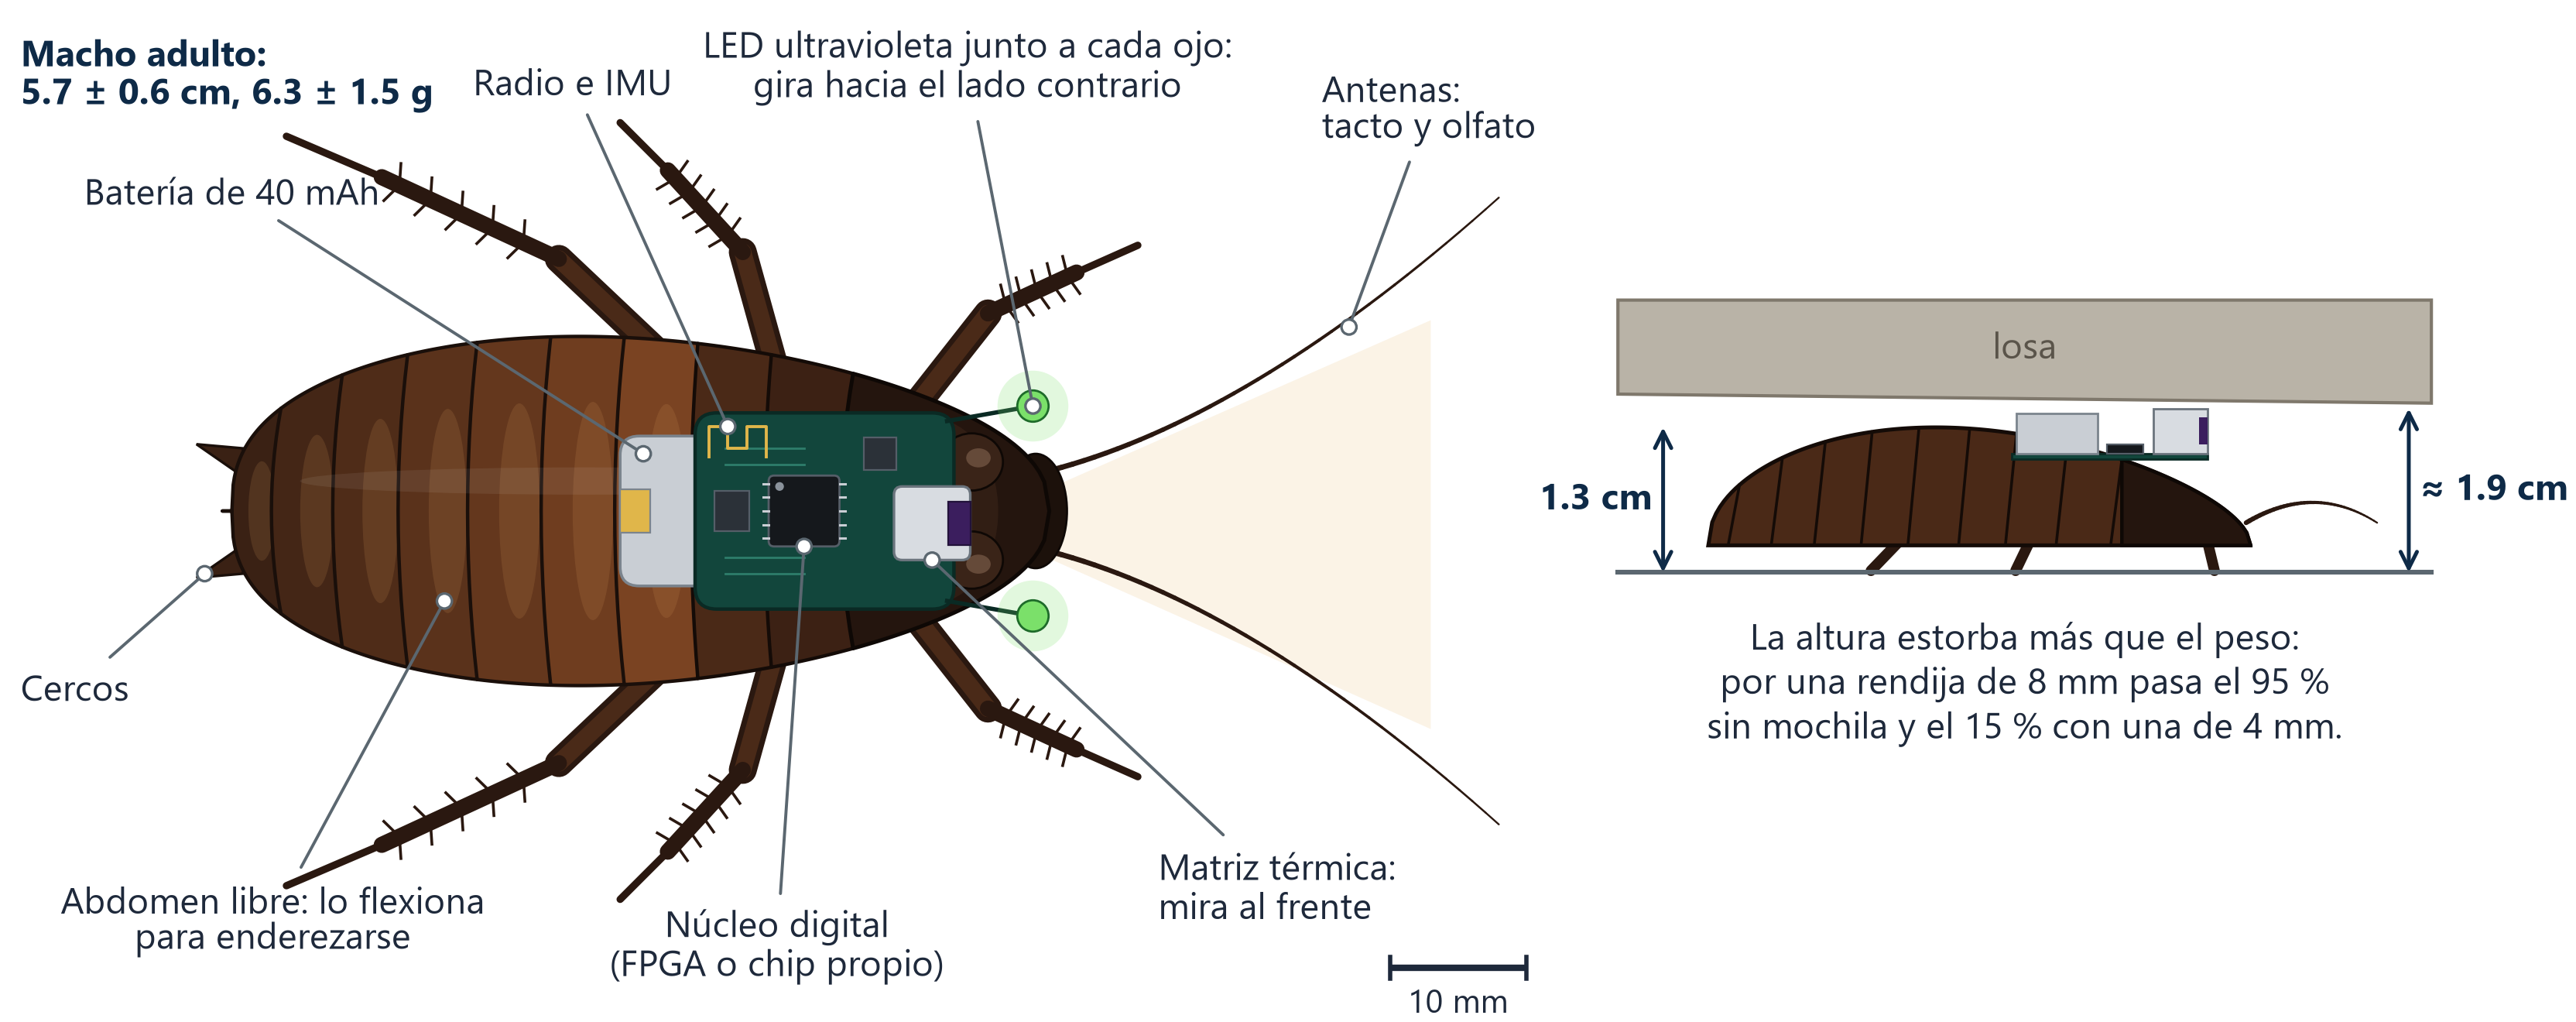
\includegraphics[width=0.74\textwidth]{insecto_mochila.png}\par
\vspace{1.1cm}
{\large
\begin{tabular}{c}
\textbf{Roberto Orozco Ramírez}\quad 184595\\[3pt]
\textbf{Adam Del Pozo Ontiveros}\quad 185611\\[3pt]
\textbf{Enrique Bernal Martín Prieto}\quad 184878
\end{tabular}}\par
\vspace{0.9cm}
{\large San Andrés Cholula, Puebla, México\\[3pt] 24 de noviembre de 2026}\par
\vfill
{\small\color{Secondary}\url{https://github.com/AdamPark7014/biobot-rescue-proyecto-final}}\par
\vspace{0.3cm}
{\color{Primary}\rule{\textwidth}{2.2pt}}
\end{titlepage}
\twocolumn
\setcounter{page}{1}}

\begin{document}
\hypersetup{pageanchor=false}
\portada
\hypersetup{pageanchor=true}
\selectlanguage{spanish}

\title{BioBot-Rescue: red de mochilas embebidas en FPGA para localizar personas atrapadas con
\textit{Gromphadorhina portentosa}}

\author{\IEEEauthorblockN{Roberto Orozco Ramírez, Adam Del Pozo Ontiveros y Enrique Bernal Martín Prieto}
\IEEEauthorblockA{Universidad de las Américas Puebla\\
San Andrés Cholula, Puebla, México}}

\maketitle
\thispagestyle{plain}
\pagestyle{plain}

\begin{abstract}
Después de un sismo hay personas que quedan en huecos a los que no llega un perro, una cámara ni un robot. En este trabajo
presentamos el sistema digital de una mochila para que la cucaracha silbadora de Madagascar ayude a buscarlas, y la red con la
que varias mochilas le avisan a un operador. El núcleo cuenta los píxeles calientes de una matriz térmica y decide con una
máquina de ocho estados y un presupuesto de estímulos. Ocupa 477 elementos lógicos y dio lo mismo que su modelo de referencia en
11\,424 cuadros. Con él armamos una red de tres FPGA unidas por UART con CRC-16, número de secuencia y retransmisión. Cada nodo
reconoce a sus vecinos con filtros de Goertzel y calcula distancias exactas con una raíz entera, y el receptor triangula a la
persona con un CORDIC: se equivoca 6.2~cm a 31.95~m, en 1.10~s, y la computadora no hace ninguna cuenta. La red pasó nueve
escenarios de prueba. También llevamos el núcleo a un layout en SKY130 de 0.050~mm$^2$, sin errores de DRC ni de LVS, que consume
0.58~mA a 1.8~V y 50~MHz. En 320 misiones simuladas por caso, guiar a diez insectos sube la detección en una hora de 58 a 73~\%.
El sensor y los tonos están simulados dentro de la FPGA y no hicimos pruebas con insectos.
\end{abstract}

\begin{IEEEkeywords}
FPGA, insecto cíborg, búsqueda y rescate, CORDIC, filtro de Goertzel, CRC-16, triangulación, SKY130.
\end{IEEEkeywords}

\begin{otherlanguage}{english}
\renewcommand{\abstractname}{Abstract}
\begin{abstract}
After an earthquake, people get trapped in voids that dogs, cameras and robots cannot reach. We present the digital system of a
backpack that lets the Madagascar hissing cockroach help find them, and the network that several backpacks use to report to one
operator. The core counts the hot pixels of a thermal array and decides with an eight-state machine and a stimulus budget; it uses
477 logic elements and gave the same result as its reference model in 11,424 frames. Around it we built a network of three FPGAs
linked by UART, with CRC-16, sequence numbers and relaying. Each node detects its neighbors with Goertzel filters and computes exact
distances with an integer square root, and the receiver locates the person with a CORDIC: the error is 6.2~cm at 31.95~m in 1.10~s,
and the host computes nothing. We also took the core to a 0.050~mm$^2$ SKY130 layout, DRC and LVS clean, that draws 0.58~mA at 1.8~V
and 50~MHz. In 320 simulated missions per case, guiding ten insects raises one-hour detection from 58 to 73\%. The sensor and the
tones are simulated inside the FPGA, and we did not test with insects.
\end{abstract}
\end{otherlanguage}

\section{Introducción}

En un derrumbe el tiempo para sacar a alguien con vida es corto. De las personas liberadas el primer día en Kobe (1995) sobrevivió cerca
del 80~\%, y a partir del cuarto día, casi nadie~\cite{kawata}. Los datos de Italia (1980) son parecidos: de los atrapados que
sobrevivieron, al 93~\% lo sacaron en las primeras 24~h~\cite{noji}. El tema nos queda cerca, porque el sismo del 19 de septiembre de 2017,
entre Puebla y Morelos, dejó 369 muertos y 44 edificios colapsados en la Ciudad de México~\cite{galvis2020}. Los huecos que se
exploraron en el World Trade Center eran, por lo general, de menos de 1~m~\cite{murphy2004}, y hasta 2021 ningún robot terrestre
había encontrado a una persona viva en un desastre~\cite{murphy2021}.

La cucaracha silbadora de Madagascar (\textit{Gromphadorhina portentosa}) puede ayudar ahí. Mide 6~cm de largo y 1.3~cm de alto, se trepa a obstáculos de su tamaño y suele ir pegada a las paredes. Ya hay
grupos que le montan sensores~\cite{tranngoc2023,lin2025,refat2025}, y en 2025 se llevó por primera vez a un desastre, en Myanmar,
aunque no se halló a nadie con vida~\cite{htx2025}. Nosotros buscábamos algo que no vimos reunido en esos trabajos: que no hubiera cirugía, que
nadie tuviera que pilotear, que el circuito cupiera en los 2 a 3~g que carga el animal y que el rescatista supiera \emph{dónde} está la
persona, incluso si el insecto que la encontró ya salió del alcance de la radio.

La figura~\ref{fig:sistema} resume la idea. Se deja que el insecto explore a su modo, la mochila lo estimula poco y transmite únicamente
si detecta algo, y un relevo en la entrada pasa el aviso a la estación, que indica dónde cavar.

\begin{figure}[!tb]
\centering
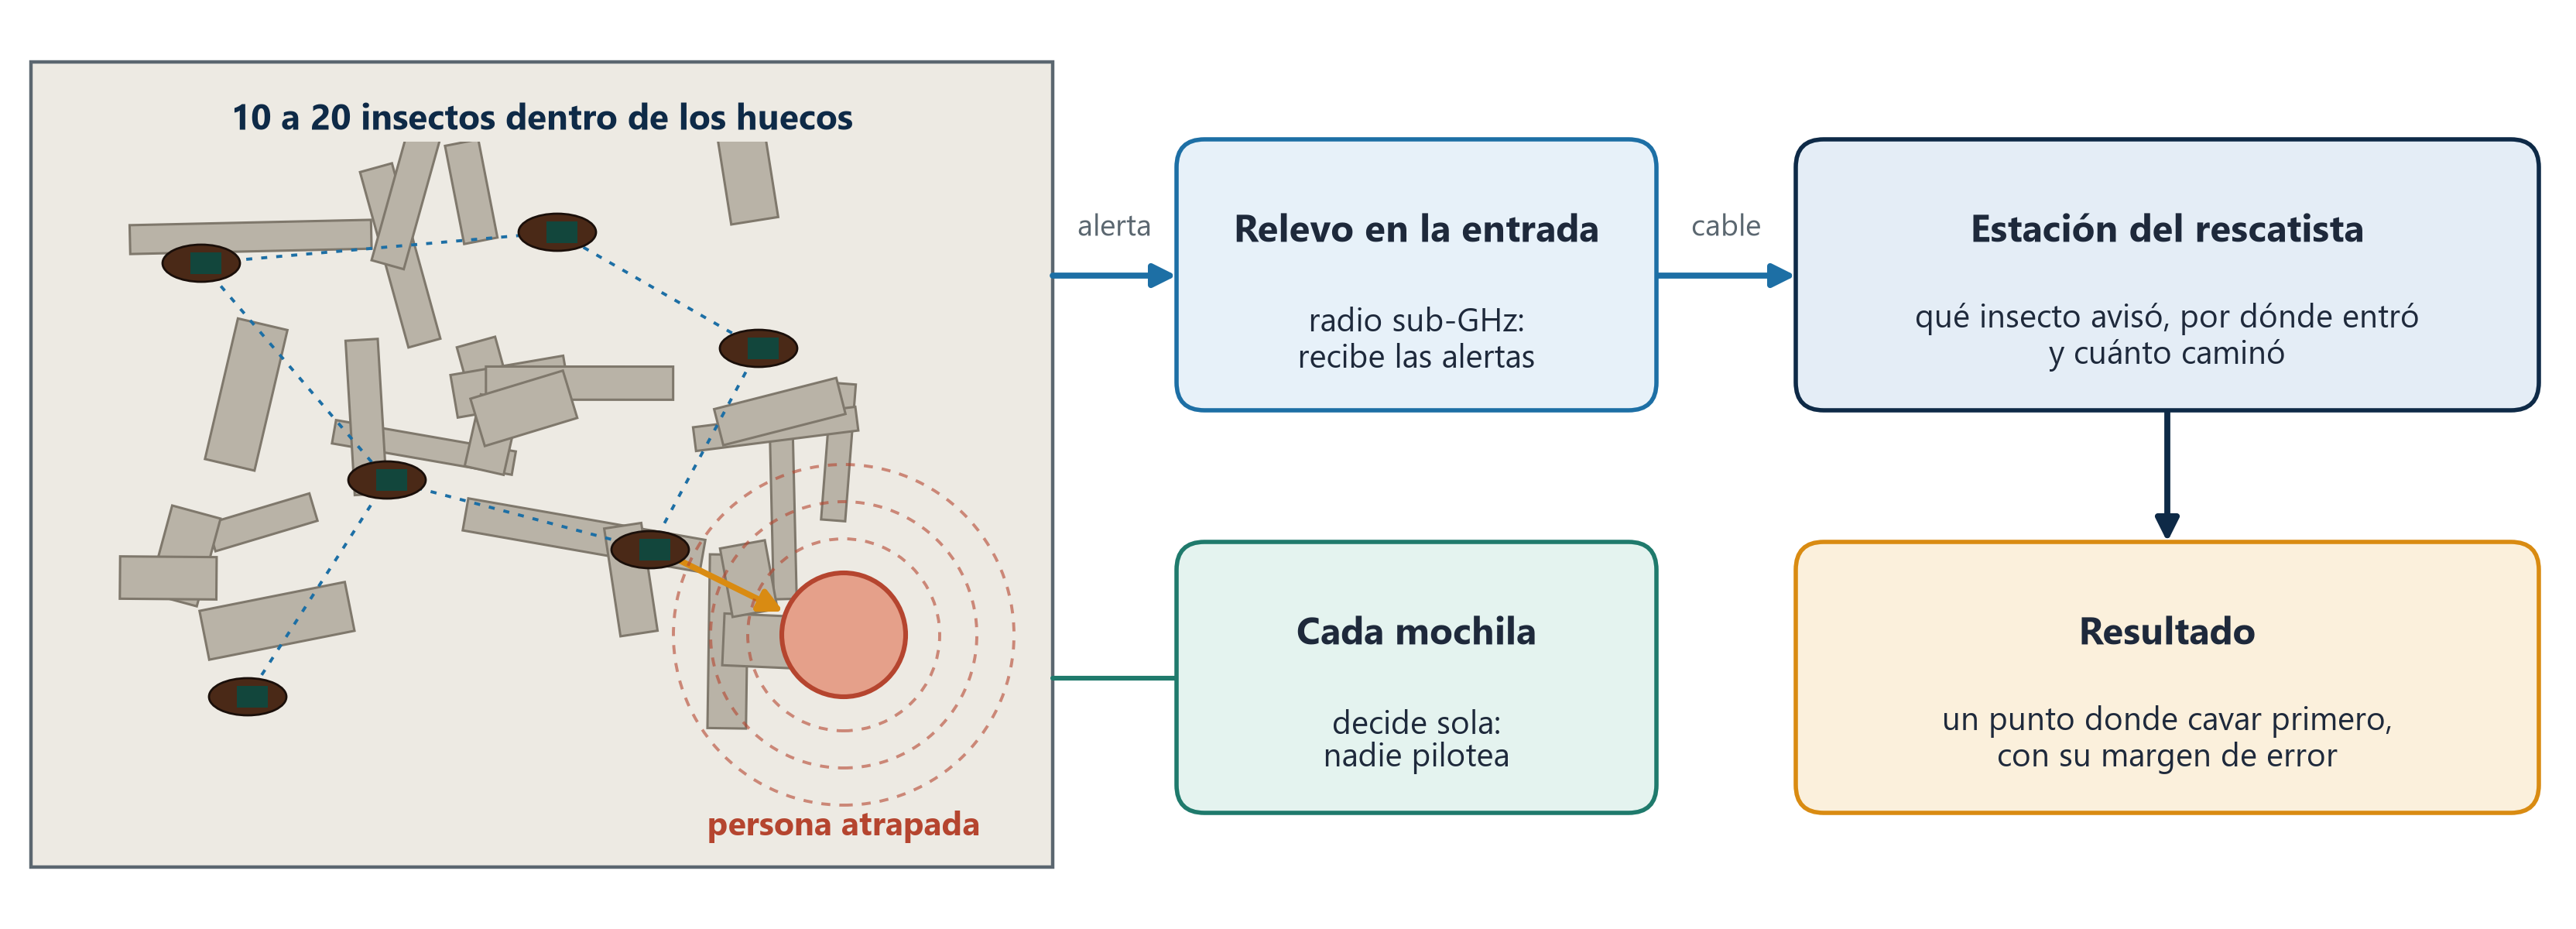
\includegraphics[width=\columnwidth]{sistema.png}
\caption{Sistema completo: de los insectos en los huecos al punto que el rescatista debe revisar primero.}
\label{fig:sistema}
\end{figure}

Lo que presentamos es:
\begin{itemize}
\item un núcleo digital que cierra el lazo a bordo (detección, decisión y estímulo) en 477 elementos lógicos, que comparamos cuadro
      por cuadro con un modelo y probamos en dos tarjetas;
\item una red de tres FPGA que detecta, retransmite y triangula sin que la computadora calcule nada;
\item cuánto se equivoca cada bloque en punto fijo, y la comparación que nos hizo cambiar el CORDIC por una raíz entera para las
      distancias;
\item un layout del núcleo en SKY130 con su área y su consumo de corriente por esquina;
\item una evaluación de la misión, en la que incluimos el caso en que guiar empeora el resultado.
\end{itemize}

\section{Trabajos relacionados}

Latif y Bozkurt~\cite{latif2012} dirigieron a \Gp{} por control remoto con electrodos en las antenas. Erickson
\textit{et al.}~\cite{erickson2015} mostraron que el pulso monofásico habitúa y el bifásico no; Sanchez
\textit{et al.}~\cite{sanchez2015} midieron recuperación con 10~min de descanso, y Ma \textit{et al.}~\cite{ma2023}, una
caída del 57~\% tras diez estímulos. El grupo de NTU logró 94~\% de éxito entre muros y detección de personas con una
matriz de $32\times32$~\cite{tranngoc2023}, electrodos sin cirugía~\cite{lin2023} y ensamble
robotizado~\cite{lin2025}; con Osaka, un enjambre de veinte insectos coordinado por una computadora~\cite{bai2025}. Refat \textit{et al.}~\cite{refat2025} guían con luz ultravioleta y no vieron habituación en 150 ensayos. En nuestra universidad ya se
midió que la actividad es máxima cerca de 30~\textdegree C y que esa luz aumenta la locomoción~\cite{gracidas2026}.

En la tabla~\ref{tab:cmp} resumimos las diferencias. Casi toda la navegación publicada se apoya en cámaras externas o en una computadora. Tampoco vimos que alguien cruzara lo que detectan dos mochilas
para ubicar a la persona, o que una le sirviera de relevo a otra. Y manejar un enjambre desde un solo operador ya se había descartado por
«físicamente impráctico»~\cite{murphy2004}. Nuestra salida fue quitar al piloto y dejar que la mochila decida y avise por su cuenta.

\begin{table}[!tb]
\centering\tabfont
\caption{Este trabajo frente a los sistemas publicados}
\label{tab:cmp}
\begin{tabularx}{\columnwidth}{@{}l>{\raggedright\arraybackslash}X>{\raggedright\arraybackslash}Xcc@{}}
\toprule
Trabajo & Cómputo & Quién decide & Det. & Varias \\
\midrule
\cite{latif2012} & Microcontrolador & Operador & No & No \\
\cite{tranngoc2023} & Cortex-M4F & Detección a bordo; posición externa & Sí & No \\
\cite{bai2025} & Módulo inalámbrico & Computadora & No & Navegar \\
\cite{refat2025} & Casco con luz & Autónomo & No & No \\
\textbf{Propuesto} & FPGA o 0.050~mm$^2$ & A bordo, con presupuesto & Sí & Ubicar \\
\bottomrule
\end{tabularx}
\end{table}

\section{El núcleo de la mochila}

\subsection{Restricciones del portador}

Lo primero fue saber cuánto se le puede cargar. Con 15~g el insecto se detiene~\cite{montagut2024} y con 4~g ya se controla
peor~\cite{latif2012}, así que limitamos la mochila a 2--3~g. Camina a 1.9~cm/s, pasa quieto cerca del 60~\% del
tiempo~\cite{dirafzoon2017} y tras un estímulo avanza a unos 5~cm/s~\cite{tranngoc2024}. Como estímulo elegimos la luz ultravioleta,
que no requiere cirugía ni habitúa. Modelamos la respuesta con probabilidad $p(1-H)$, $p=0.78$~\cite{lin2023}, y
\begin{equation}
H\leftarrow H+\alpha(1-H),\qquad H(t+\Delta t)=H(t)\,e^{-\Delta t/\tau},
\end{equation}
con $\tau=600$~s~\cite{sanchez2015}.

\subsection{Detección}

Con un solo píxel de campo amplio casi no se nota que hay una persona. A medio metro de una cara, con fondo de 22~\textdegree C, lee
22.4~\textdegree C, porque promedia toda la escena. Con una matriz ya no pasa, ya que un blanco de área $A$ a distancia $d$ ocupa
$n=A/(d\tan\theta)^2$ píxeles. El módulo \sig{ventana\_termica} recibe los 64 píxeles de 8~bits (0.25~\textdegree C por cuenta) y
cuenta como caliente el que está entre 28 y 38~\textdegree C~\cite{tranngoc2023} y además supera en 2~\textdegree C la media del
cuadro anterior; también dice de qué lado domina la mancha. Como el insecto se balancea al caminar, una media móvil de cuatro cuadros
quita ese vaivén. Luego \sig{detector\_presencia} pide 2 píxeles para acercarse y 8 durante cuatro cuadros para confirmar. En la
figura~\ref{fig:rtlven} se ve el circuito que resulta. Con la matriz de $8\times8$ (60\textdegree) la detección se confirma a 0.9~m y
con la de $32\times32$ (90\textdegree), a 1.25~m.

\begin{figure}[!tb]
\centering
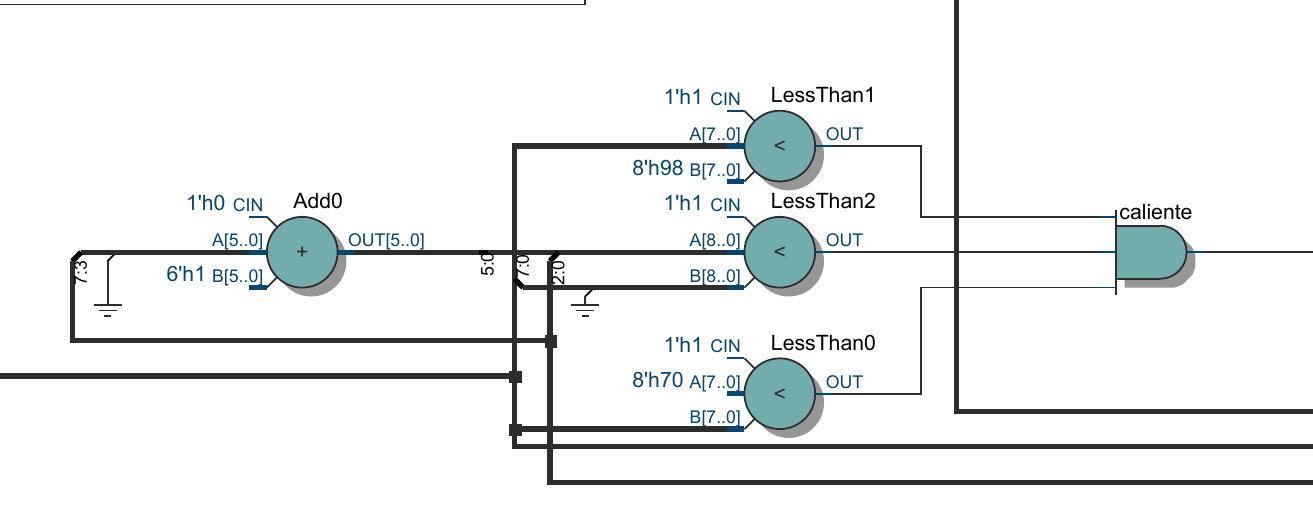
\includegraphics[width=\columnwidth]{zoom_ventana_termica.png}
\caption{Criterio de píxel caliente en el RTL Viewer: dos comparadores de ventana (\sig{8'h70} = 28~\textdegree C,
\sig{8'h98} = 38~\textdegree C), el fondo más 2~\textdegree C y la compuerta \sig{caliente}.}
\label{fig:rtlven}
\end{figure}

\begin{figure*}[!t]
\centering
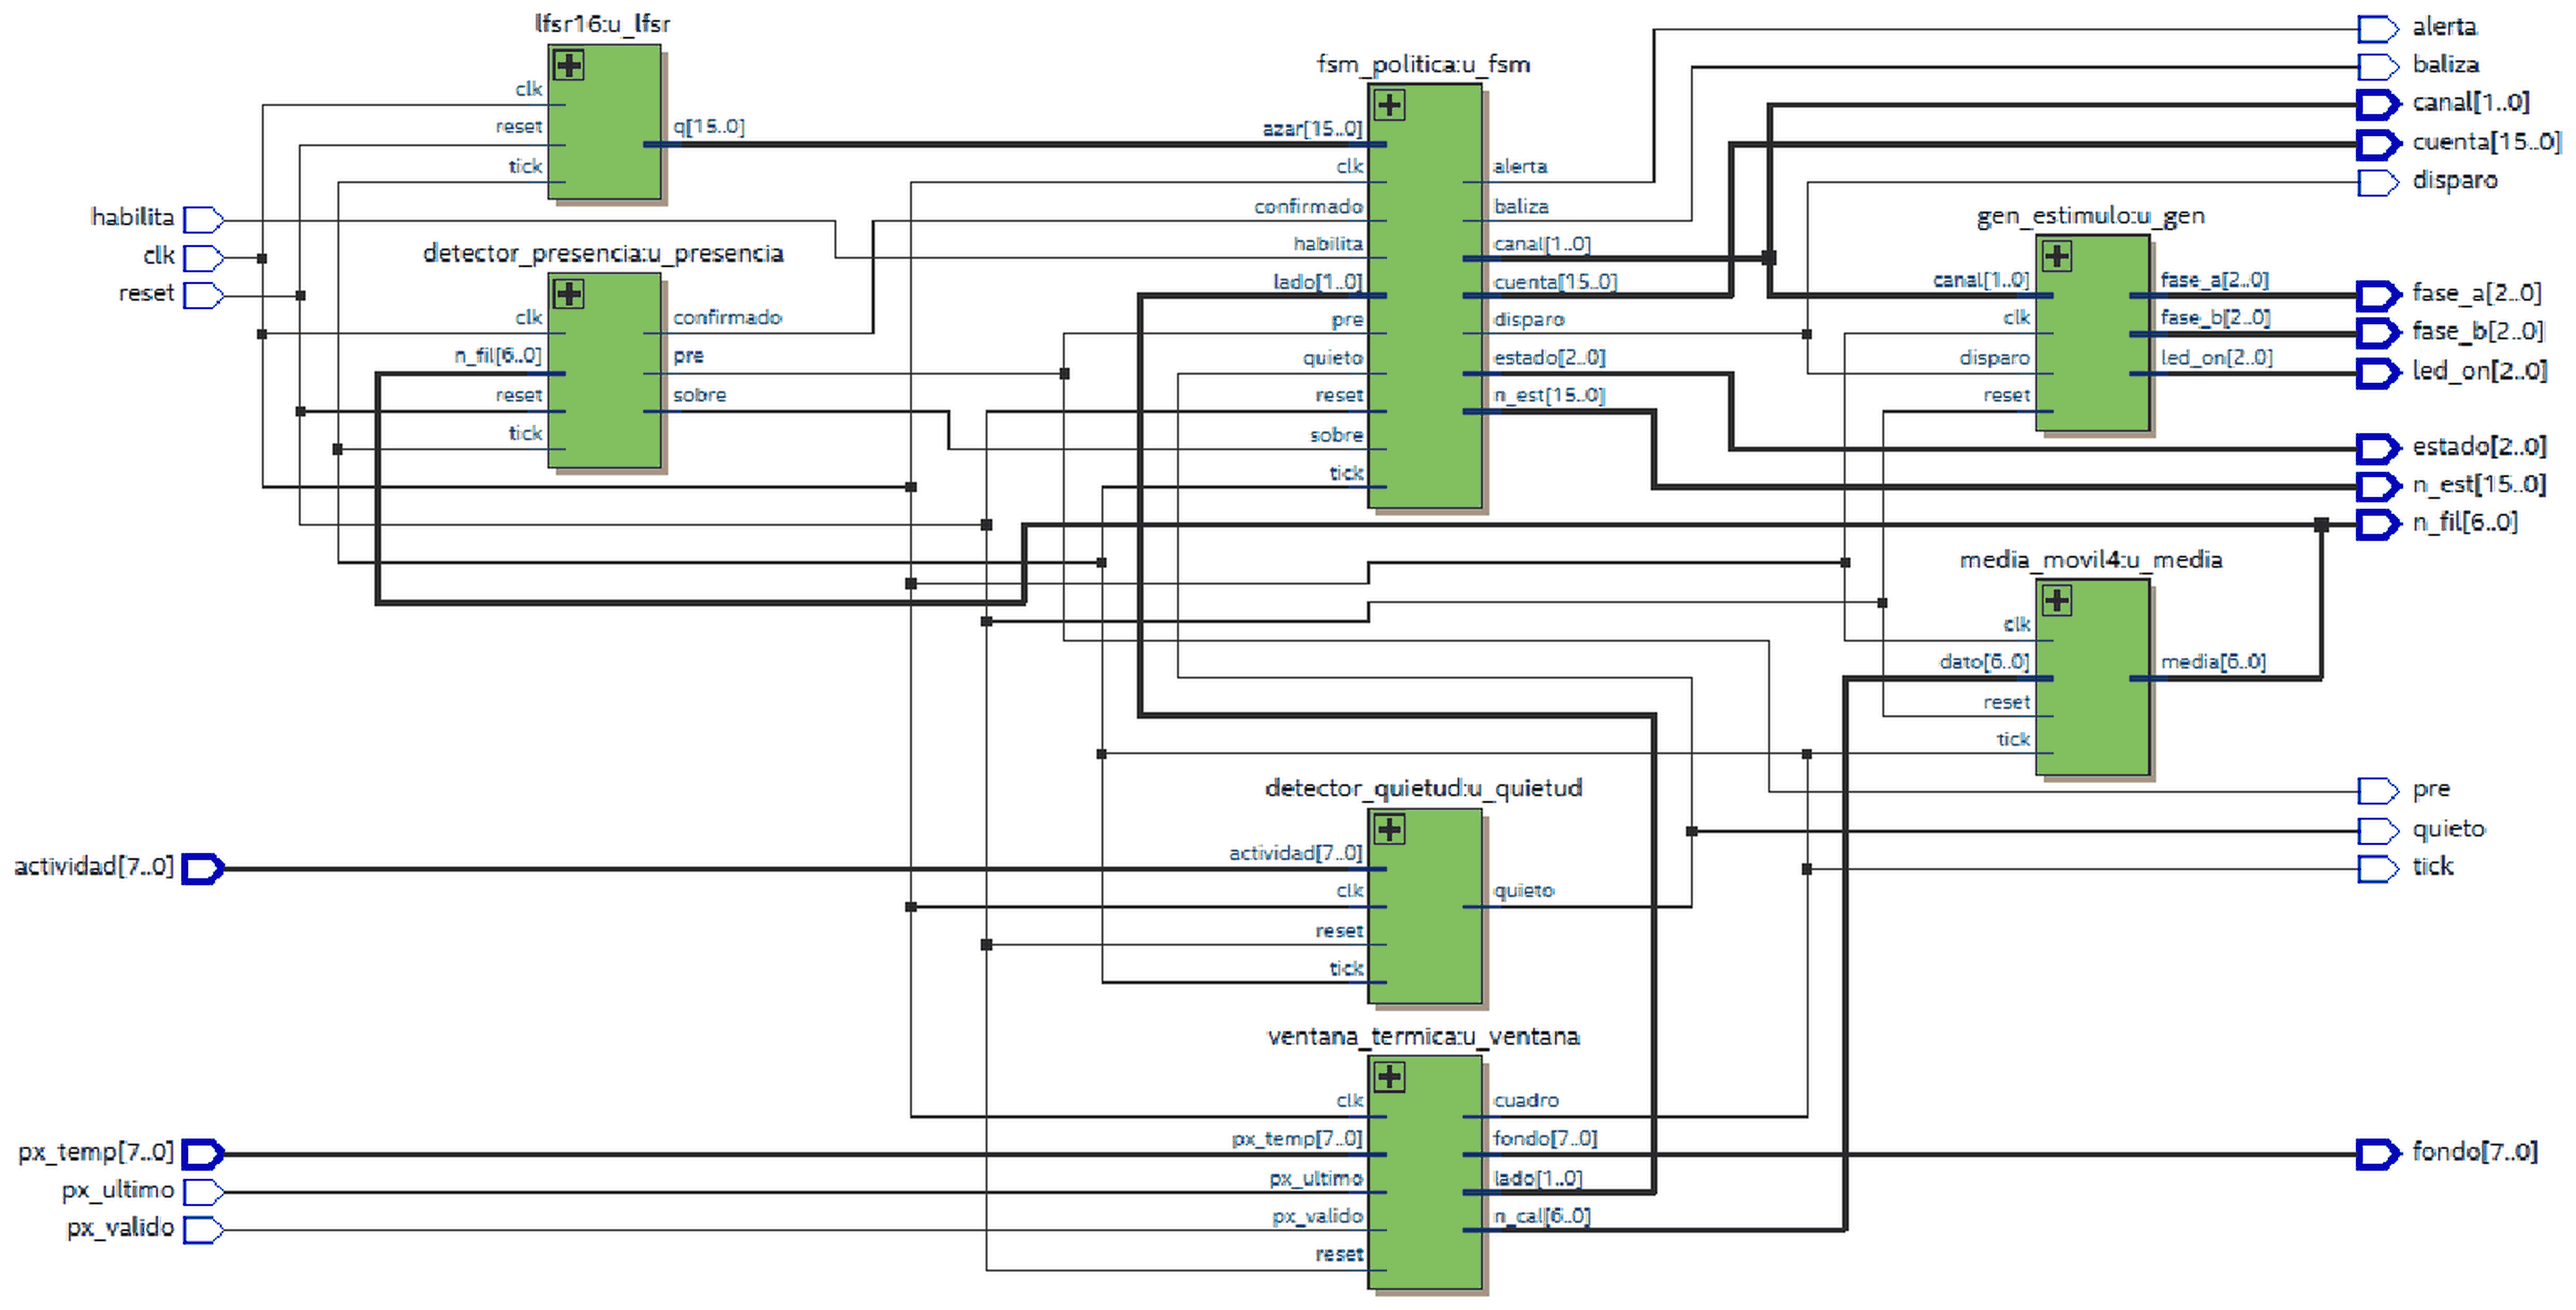
\includegraphics[width=0.80\textwidth]{rtl_nucleo.png}
\caption{Núcleo de la mochila tal como lo sintetiza Quartus (RTL Viewer): ventana térmica, media móvil, detectores de
presencia y de quietud, generador seudoaleatorio, máquina de estados y generador de estímulo.}
\label{fig:rtl}
\end{figure*}

\subsection{Política de estímulo}

La máquina \sig{fsm\_politica} (fig.~\ref{fig:rtl}) avanza una vez por cuadro, diez veces por segundo, por ocho estados:
reposo, explorar, reactivar, reorientar, acercar, confirmar, alertar y descanso. No es un control remoto, porque nadie le dice cuándo estimular. La primera de sus tres reglas es una espera que se duplica: tras 15~s quieto da un pulso de avance
y, si en 3~s no arranca, espera 30, 60 y 120~s. La segunda son giros al azar, que un LFSR de 16~bits dispara cada 51~s en promedio para
despegar al insecto de las paredes~\cite{dirafzoon2017}. La tercera es un presupuesto. Cada estímulo suma 1 a una cuenta Q8.8 que pierde
$1/256$ cada 2.3~s ($\tau\approx590$~s, cercana a la recuperación del insecto), y con 12 acumulados deja de estimular. Así acotamos la
habituación sin tener que medir la respuesta. El módulo \sig{gen\_estimulo} produce trenes bifásicos de 50~Hz y 0.5~s. Los estados están
en la figura~\ref{fig:fsm}.

\begin{figure}[!tb]
\centering
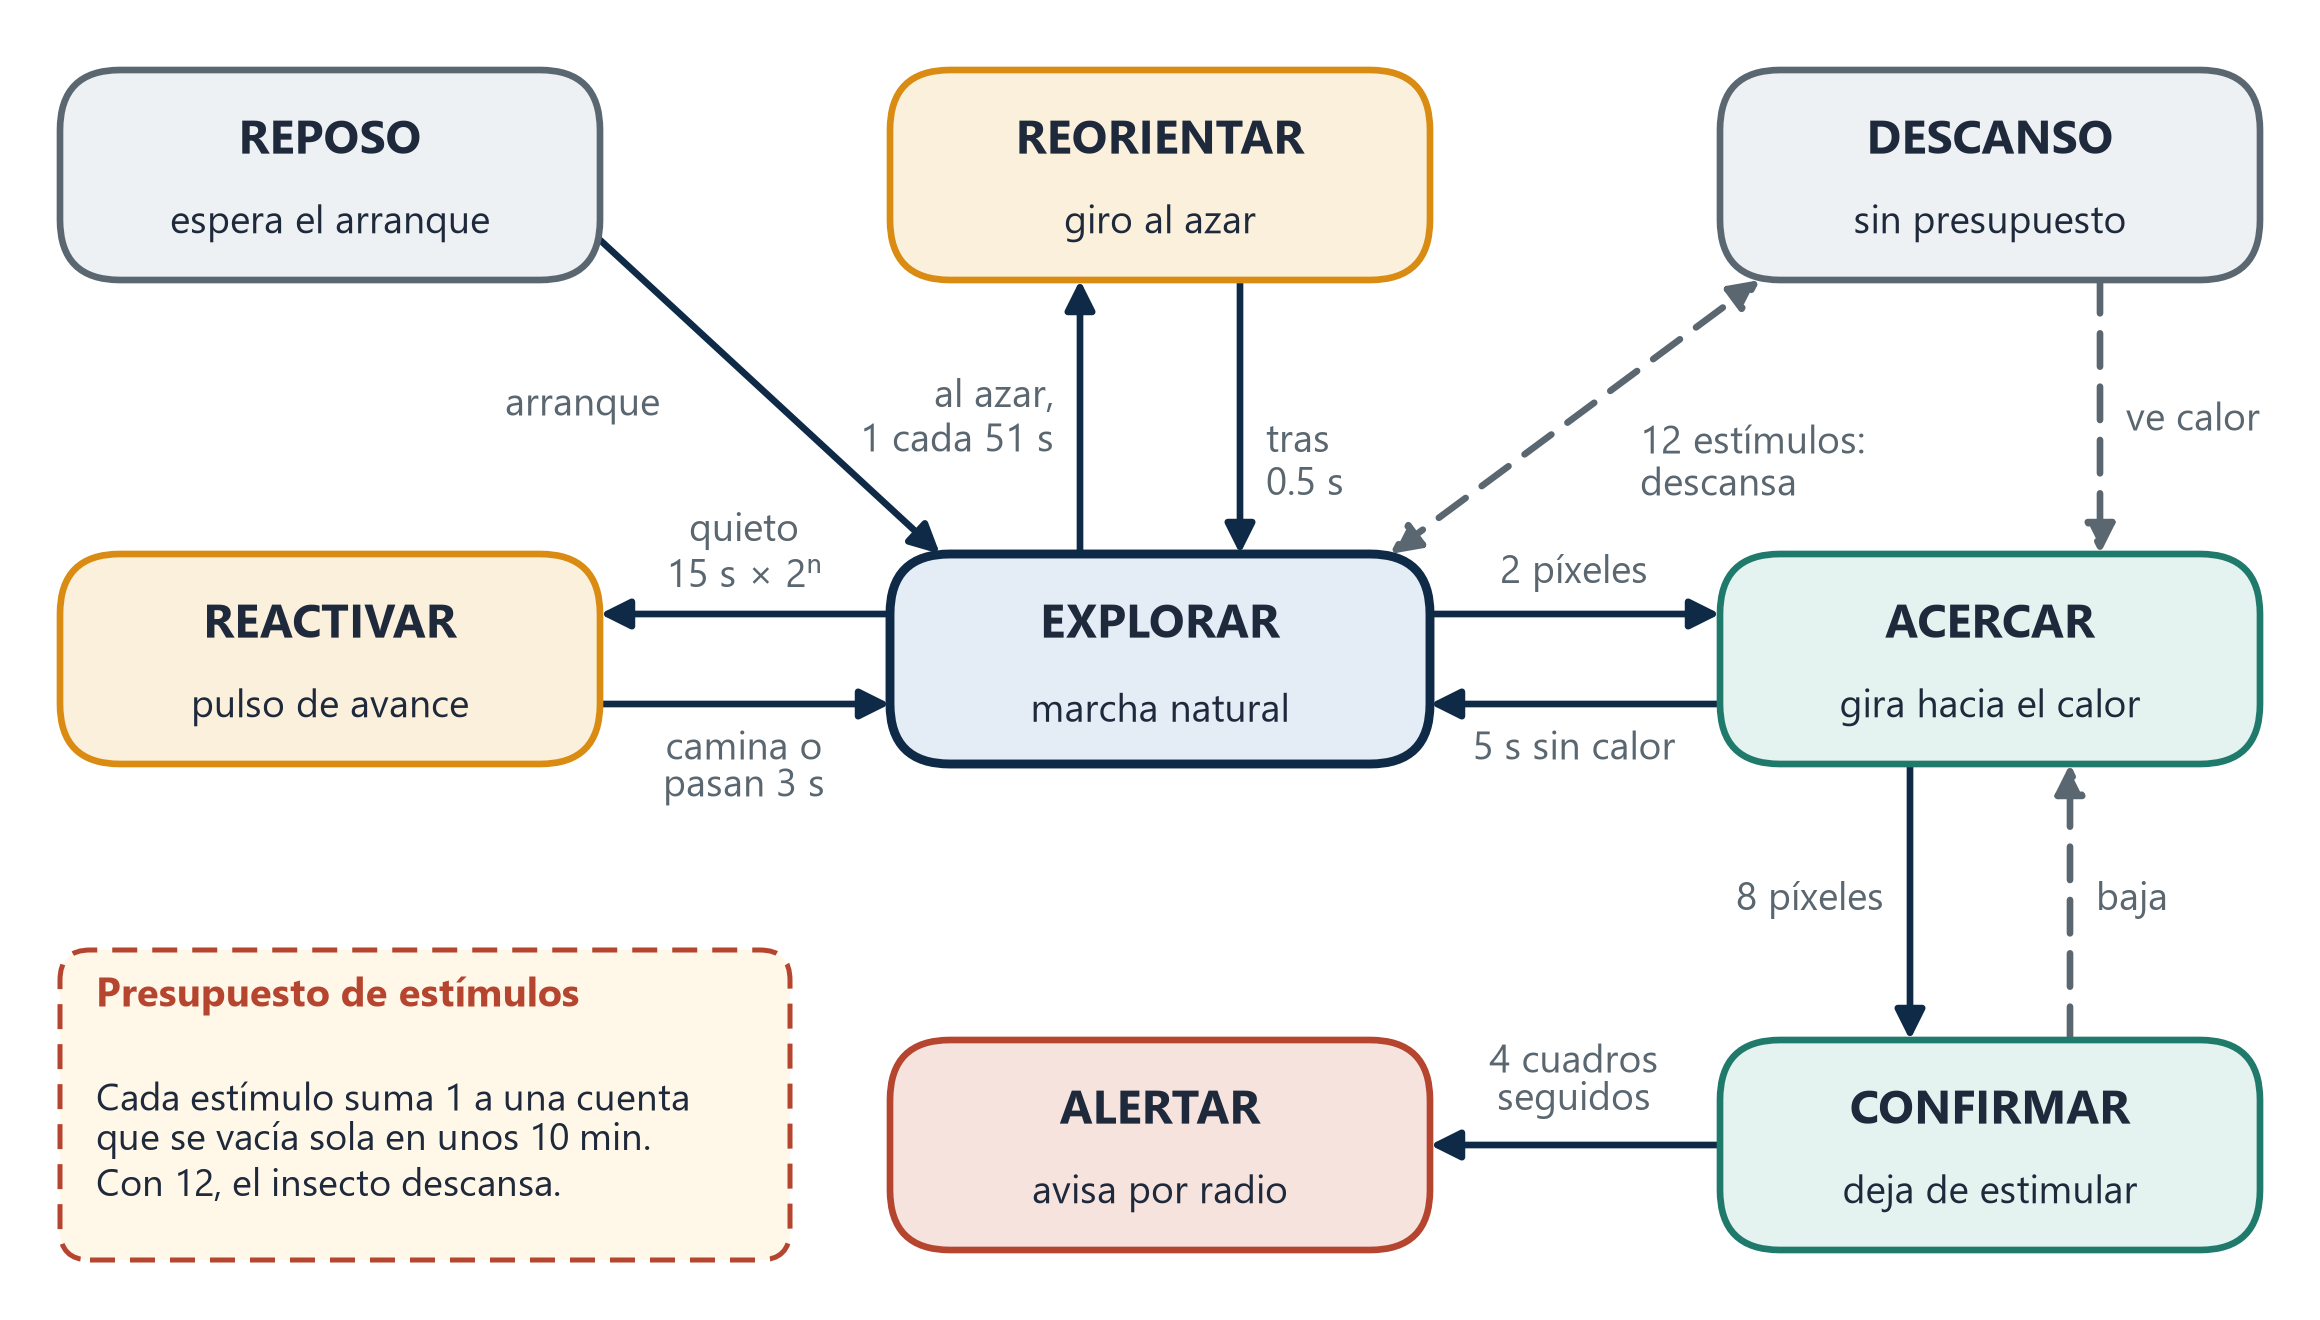
\includegraphics[width=\columnwidth]{fsm_politica.png}
\caption{Máquina de estados de la política. Las flechas punteadas no producen estímulo.}
\label{fig:fsm}
\end{figure}

\section{La red de tres nodos}

\begin{figure*}[!t]
\centering
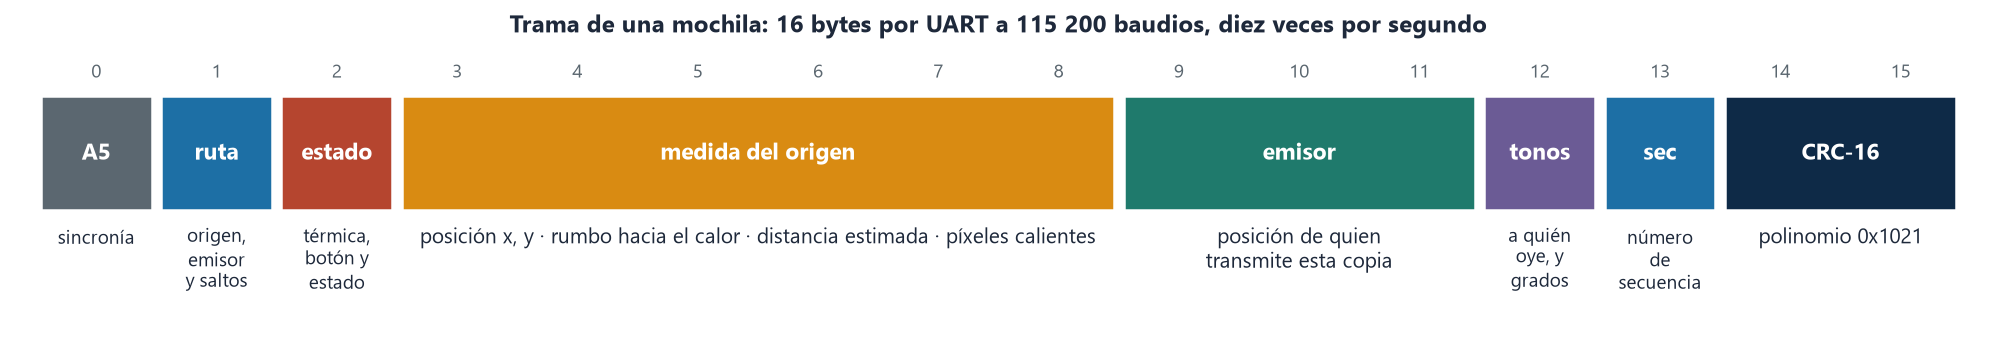
\includegraphics[width=0.86\textwidth]{red_trama.png}
\caption{Trama de 16 bytes de una mochila.}
\label{fig:trama}
\end{figure*}

\begin{table*}[!t]
\centering\tabfont
\caption{Módulos principales: función, recursos en MAX~10 y latencia}
\label{tab:mod}
\renewcommand{\sig}[1]{{\footnotesize\texttt{#1}}}
\begin{tabularx}{\textwidth}{@{}l>{\raggedright\arraybackslash}Xrrl@{}}
\toprule
Módulo & Función & EL & Reg. & Latencia \\
\midrule
\sig{ventana\_termica} & Cuenta píxeles calientes, lado de la mancha y media del cuadro & 160 & 61 & 1 ciclo tras el último píxel \\
\sig{media\_movil4} & FIR de cuatro coeficientes iguales & 40 & 28 & 1 cuadro \\
\sig{detector\_presencia} & Umbrales de 2 y 8 píxeles con confirmación & 9 & 4 & 4 cuadros \\
\sig{detector\_quietud} & Un segundo sin actividad en la IMU & 10 & 4 & 10 cuadros \\
\sig{fsm\_politica} & Ocho estados, espera que se duplica y presupuesto & 181 & 64 & 1 cuadro \\
\sig{gen\_estimulo} & Tren bifásico de 50~Hz por tres canales & 64 & 47 & 2 ciclos \\
\sig{tri\_tx\_n}, \sig{tri\_rx\_n} & Trama con cabecera, carga y CRC-16 & 209, 370 & 172, 305 & 1.4~ms por trama \\
\sig{tri\_tonos} & Tono propio y tres filtros de Goertzel & 355 & 225 & 8~ms para decidir \\
\sig{tri\_distancia} & Raíz cuadrada entera exacta & 87--109 & 60 & 12 ciclos \\
\sig{cordic} & Rotación y vectorización, 16 iteraciones & 532 & 96 & 18 ciclos \\
\sig{tri\_triangula} & Cruce de dos rumbos con detección de errores & 1\,509 & 631 & $\approx90$ ciclos \\
\sig{tri\_mochila} & Núcleo, escena simulada, radio, vecinos y displays & 3\,605 & 2\,027 & 100~ms \\
\sig{tri\_receptor} & Seguimiento de tramas, triangulación, conteo y vistas & 4\,506 & 2\,181 & 100~ms \\
\sig{pid\_q} & PID posicional con integración condicional & 213 & 66 & 1 ciclo \\
\bottomrule
\end{tabularx}
\end{table*}

\subsection{Organización}

Usamos tres DE10-Lite, dos como mochilas (A y B) y una como receptor (fig.~\ref{fig:red}). Como no tenemos la matriz térmica, la
simulamos dentro de la FPGA. Con los interruptores fijamos la temperatura, y un CORDIC calcula en qué columna caería la mancha según la
posición del insecto, de modo que al núcleo le llegan los píxeles igual que si vinieran del sensor. Para la demostración la ventana de
detección es de 35 a 38~\textdegree C, con un botón de ayuda como segunda vía. Las posiciones van en 10~bits sobre 64~m (6.25~cm por
cuenta).

\begin{figure}[!tb]
\centering
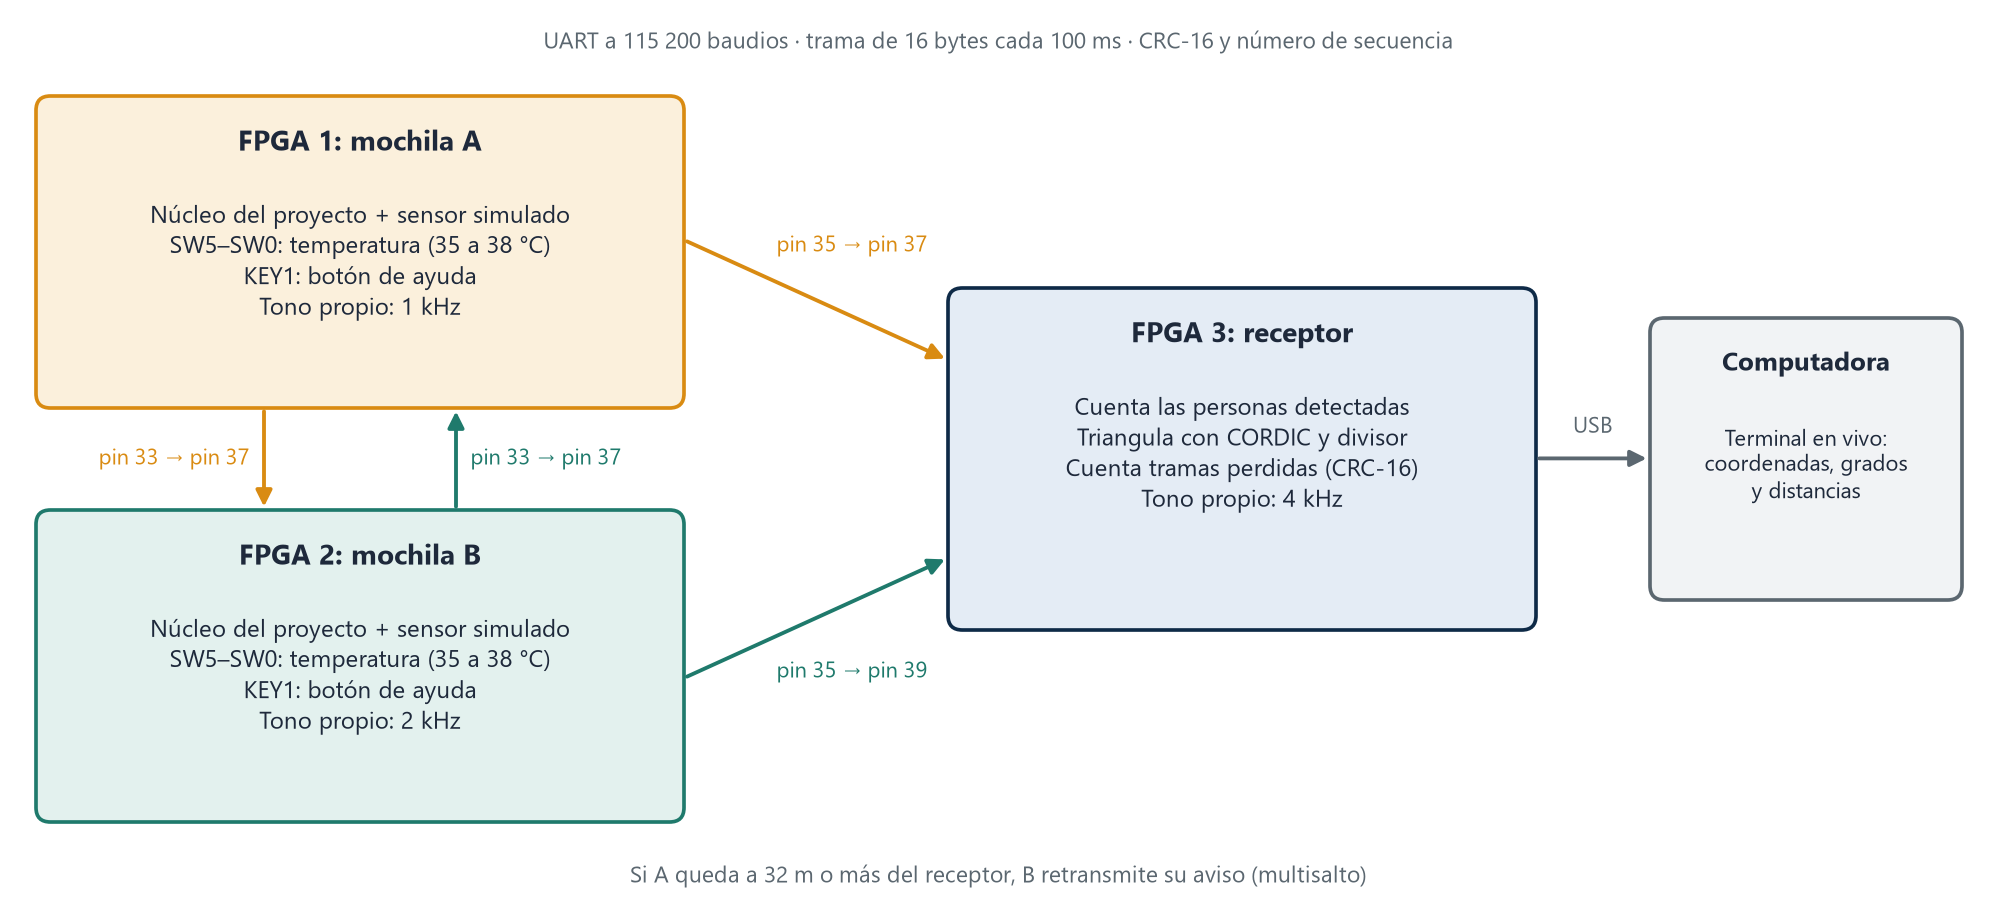
\includegraphics[width=\columnwidth]{red_tres_fpga.png}
\caption{Tres DE10-Lite: dos mochilas y el receptor. La computadora solo lee registros por JTAG.}
\label{fig:red}
\end{figure}

\subsection{Protocolo}

Cada mochila transmite cada 100~ms una trama de 16~bytes por UART a 115\,200~baudios (fig.~\ref{fig:trama}): ruta
(origen, emisor y saltos), estado, posición, rumbo, distancia estimada, número de secuencia y CRC-16 (polinomio
\sig{0x1021}), que detecta toda ráfaga de 16~bits o menos~\cite{peterson1961}. El receptor descarta las tramas corruptas o cortadas más de 2~ms y solo acepta emisores a menos de 32~m, que es como simulamos el radio.
Con el número de secuencia cuenta las perdidas y reconoce las repetidas, y si pasa 1~s sin oír a una mochila la da por perdida. Una
mochila reenvía las tramas de la otra con un salto más, así que si A quedó fuera de alcance, B hace de puente.

\subsection{Vecinos por tonos}

Cada nodo emite un tono (A 1~kHz, B 2~kHz, receptor 4~kHz) y escucha los otros dos. A 16~kHz, cada bloque de $N_b=64$
muestras pasa por tres filtros de Goertzel~\cite{goertzel1958}:
\begin{align}
s[n]&=x[n]+c\,s[n-1]-s[n-2],\quad c=2\cos(2\pi k/N_b),\\
P&=s[N_b{-}1]^2+s[N_b{-}2]^2-c\,s[N_b{-}1]\,s[N_b{-}2].
\end{align}
Escogimos esos tonos porque caen en las líneas $k=4$, 8 y 16, y así uno no se cuela en el filtro de otro. Borramos el estado en cada
bloque para que los polos sobre el círculo unitario no acumulen error. Con el tono presente la potencia va de 27\,000 a 33\,000 y sin él
no pasa de 104; pusimos el umbral en 4\,000.

\subsection{Distancia y alcance}

El módulo \sig{tri\_distancia} calcula
\begin{equation}
d=\left\lfloor\sqrt{\Delta x^2+\Delta y^2}\right\rfloor
\end{equation}
con una raíz dígito por dígito en 12 ciclos. El alcance se revisa con esa misma suma, contra $(16\cdot32)^2$, y por eso lo que marca el display siempre coincide con el corte de 32~m.

\subsection{Rumbo y triangulación}

El rumbo de cada mochila es el centroide de las columnas calientes sumado al rumbo del insecto. El receptor cruza las
dos rectas (fig.~\ref{fig:mapa}):
\begin{equation}
P=A+t\,\hat u_A,\qquad t=\frac{(B-A)\times\hat u_B}{\hat u_A\times\hat u_B}.
\end{equation}
Una máquina de ocho estados pide $\cos\theta$ y $\sin\theta$ a un CORDIC, forma los productos cruzados y divide 44 entre
32~bits, en unos 90 ciclos. No siempre hay un cruce útil. Si los rumbos difieren menos de 10\textdegree, si las rectas se cruzan detrás de una mochila o si el cruce
queda a más de 3~m, marca error y usa la aproximación de cada mochila por separado. En la figura~\ref{fig:rtltri} está el circuito y en
la tabla~\ref{tab:mod}, los módulos del sistema.

\begin{figure}[!tb]
\centering
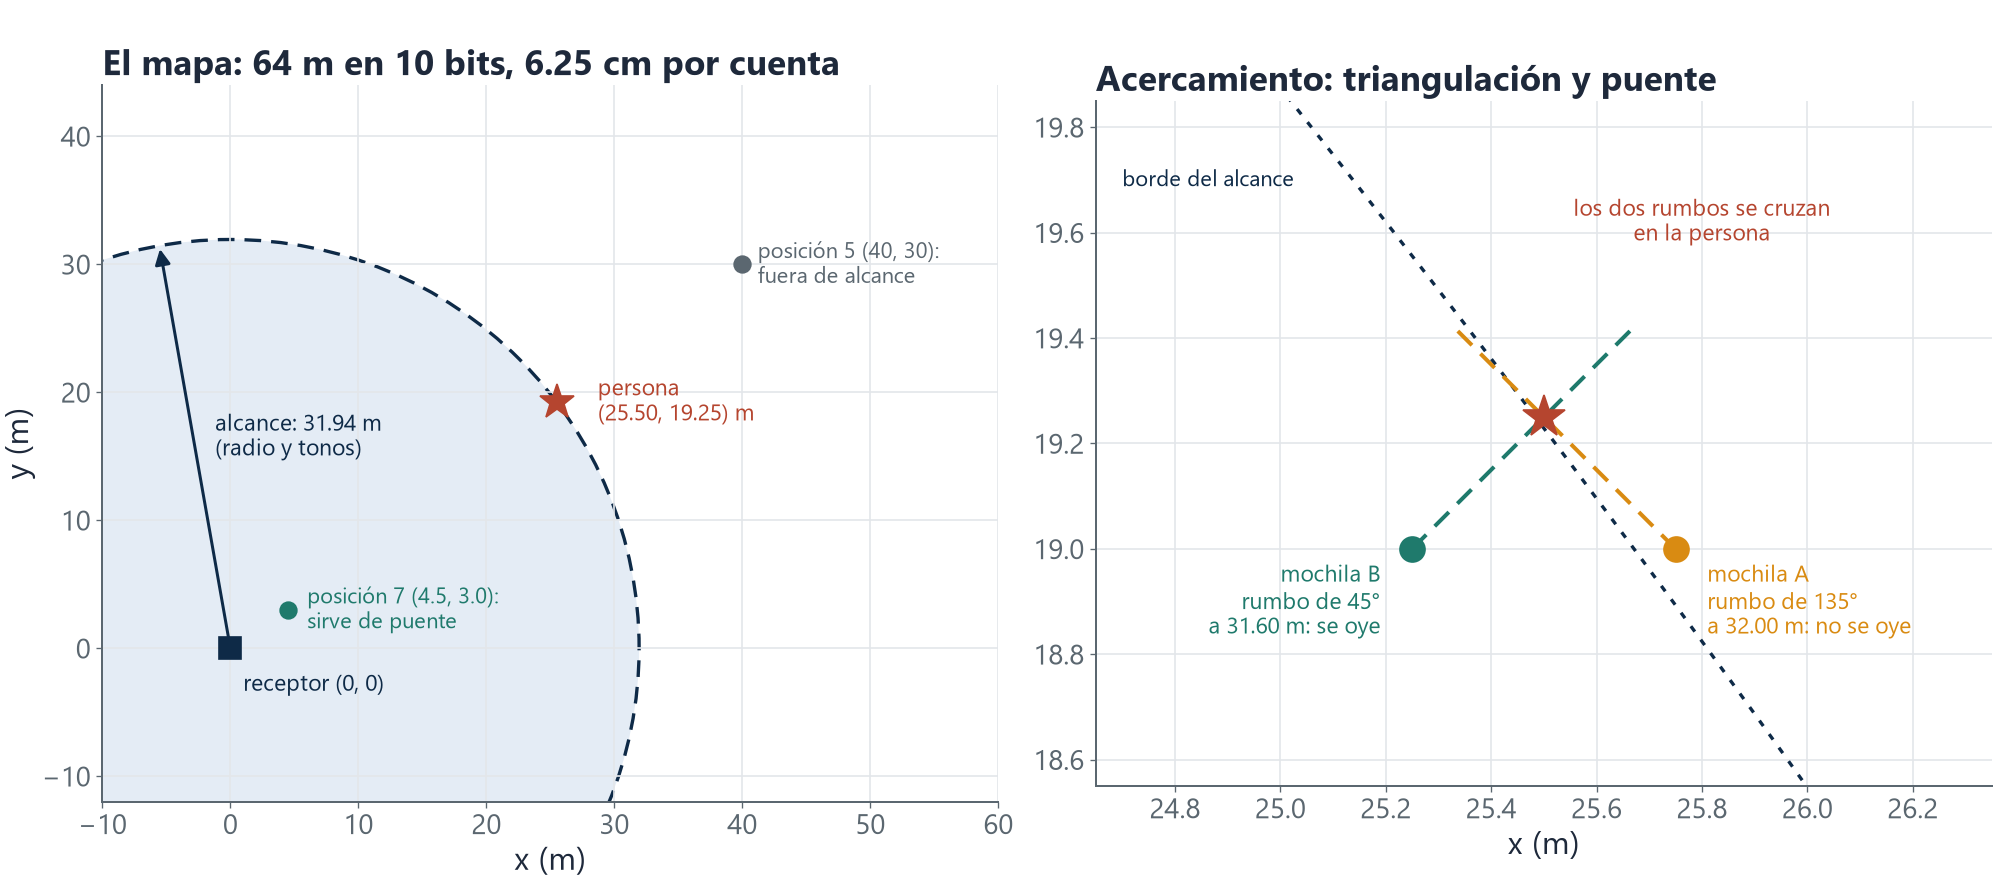
\includegraphics[width=\columnwidth]{red_mapa.png}
\caption{Mapa de 64~m con el alcance de 32~m y cruce de los dos rumbos. La persona está a 31.95~m del receptor.}
\label{fig:mapa}
\end{figure}

\section{Aritmética en punto fijo}

\begin{figure*}[!t]
\centering
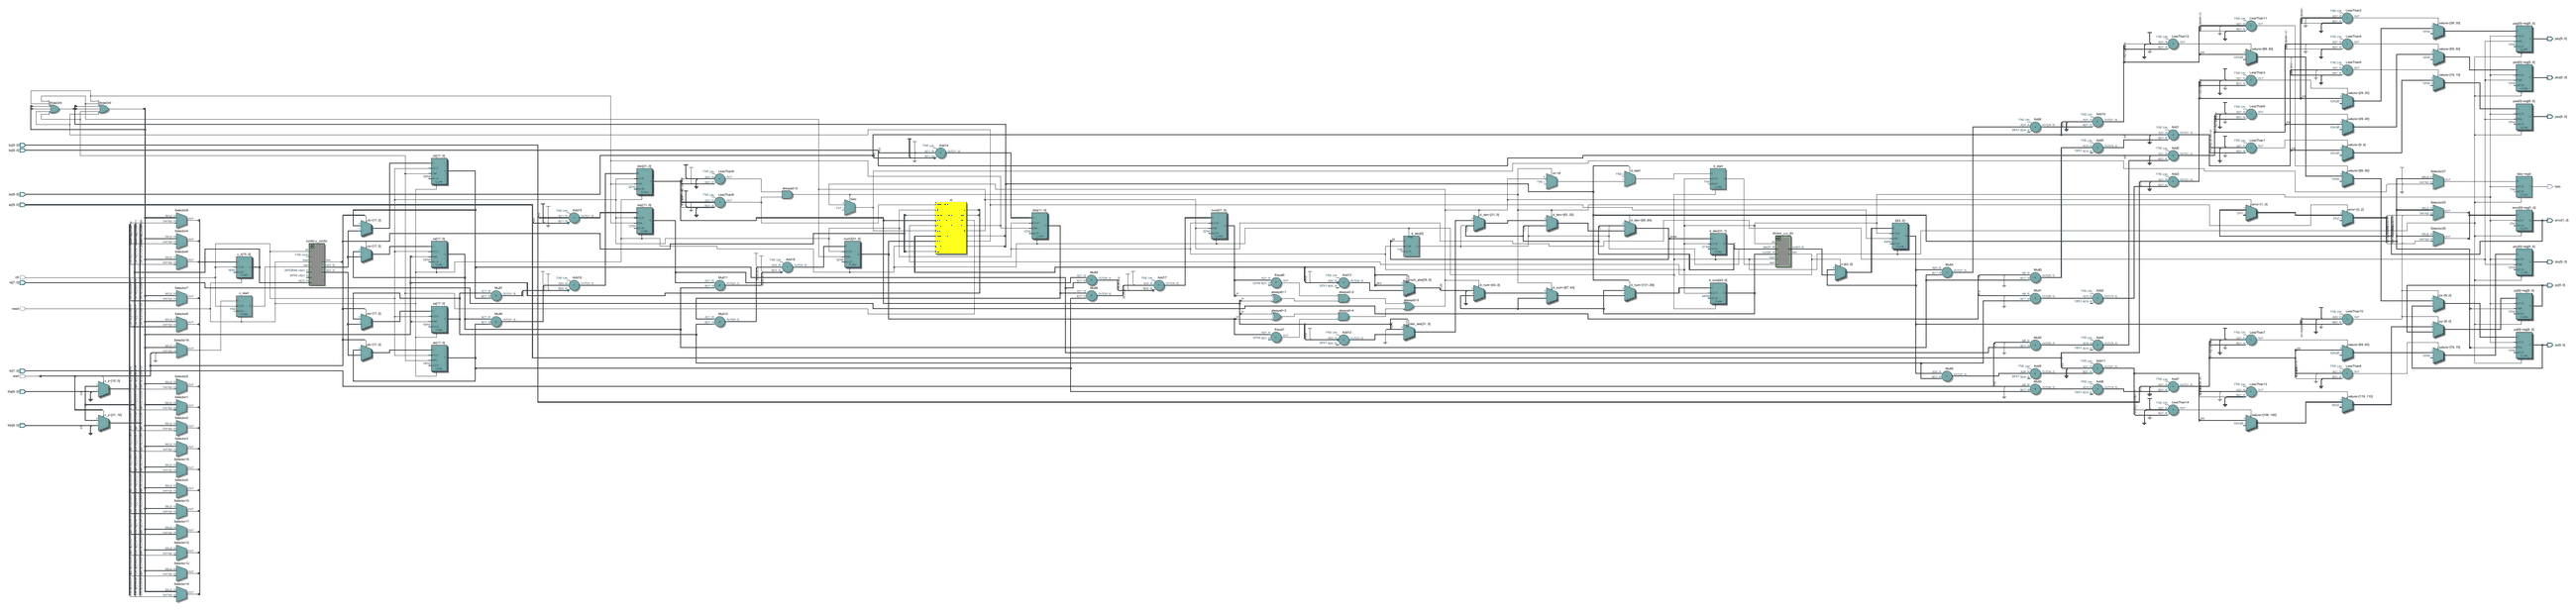
\includegraphics[width=0.98\textwidth]{rtl_tri_triangula.png}\\[3pt]
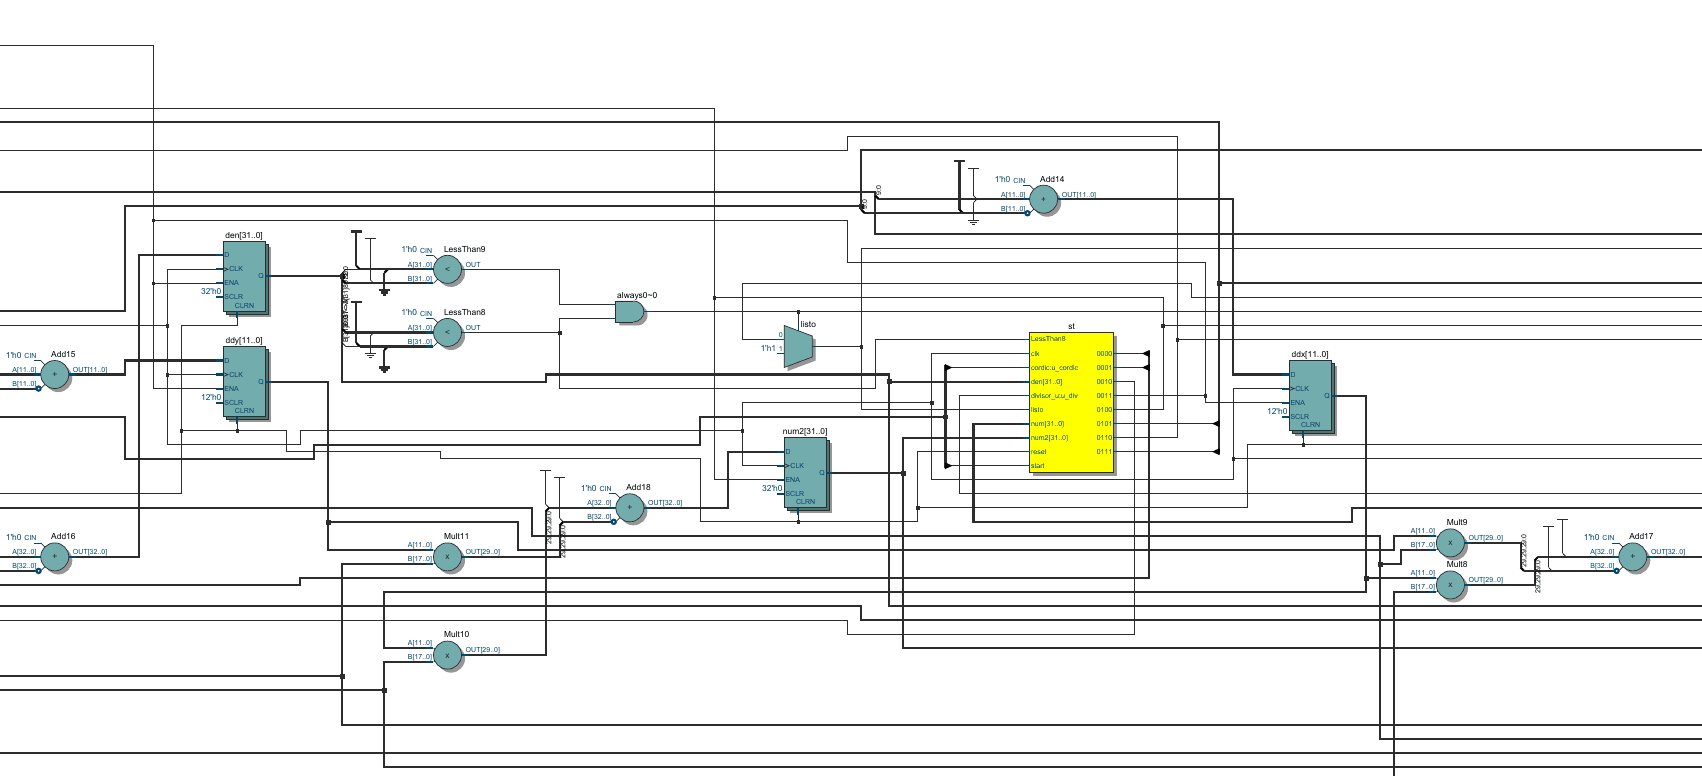
\includegraphics[width=0.62\textwidth]{zoom_tri_triangula.png}
\caption{Triangulación en el RTL Viewer. Arriba, el módulo completo, con el CORDIC y el divisor (cajas oscuras) y la máquina
de estados (amarilla). Abajo, acercamiento a los productos cruzados y a la prueba del denominador.}
\label{fig:rtltri}
\end{figure*}

El CORDIC~\cite{volder1959,andraka1998} es secuencial, de 24~bits con 4 de guarda y ángulos de 16~bits; en rotación da
seno y coseno y en vectorización, ángulo y magnitud. Para escoger el número de iteraciones comparamos nueve circuitos, de $N=4$ a 20 (fig.~\ref{fig:cordic}). El error baja
cuatro veces cada dos iteraciones hasta $N=14$, donde la tabla de arcotangentes ya no da para más. Con $N=16$ el error máximo es de
0.017\textdegree{} en el ángulo y 0.026~\% en seno y coseno.

\begin{figure}[!tb]
\centering
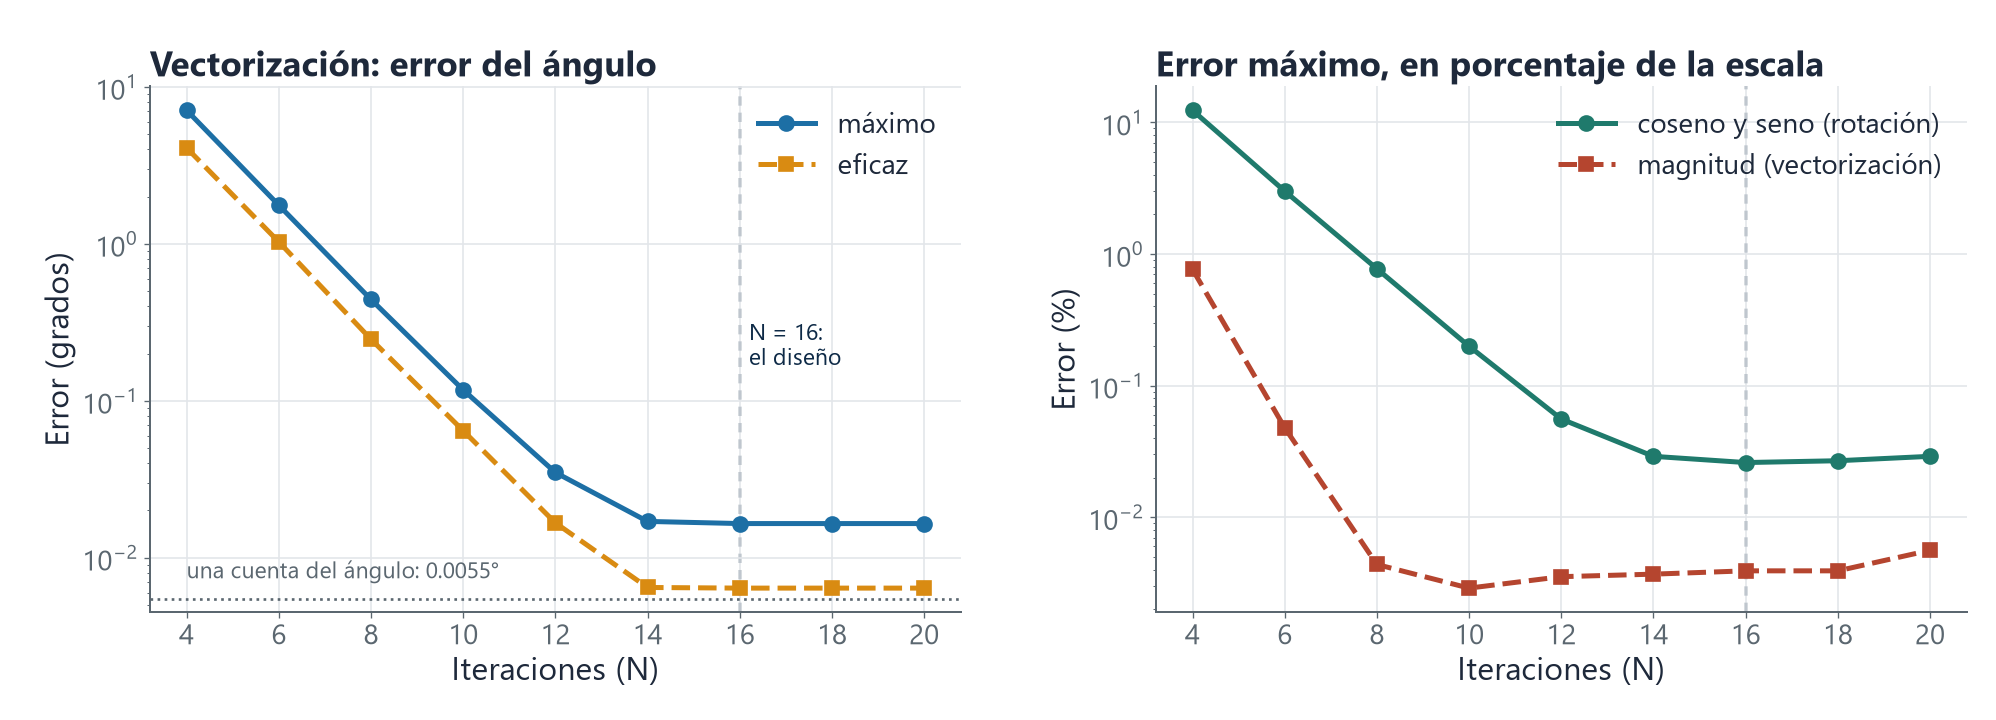
\includegraphics[width=\columnwidth]{cordic_iteraciones.png}
\caption{Error del CORDIC según el número de iteraciones, medido en la simulación del circuito con 360 vectores y 360
ángulos por valor.}
\label{fig:cordic}
\end{figure}

En la primera versión sacábamos la distancia de la magnitud del CORDIC truncada. La tabla~\ref{tab:dist} muestra por qué la cambiamos:
31.00~m sobre el eje~$Y$ se leía como 30.94~m. La raíz entera es exacta en los 1\,048\,576 pares de diferencias del mapa y ocupa la
quinta parte. Con ella la mochila bajó de 4\,812 a 3\,933 elementos lógicos. 

\textit{Filtros.} La media móvil es un FIR de fase lineal que no usa multiplicadores: tres sumas y un corrimiento, con
nulos en 2.5 y 5~Hz a diez cuadros por segundo (fig.~\ref{fig:filtros}, izquierda). Los de Goertzel son IIR de segundo
orden con coeficientes Q2.14 (30\,274, 23\,170 y 0), un error de cuantización menor que $4\times10^{-5}$ y un estado de
18~bits para una señal que no pasa de $2^{11}$.

\begin{figure}[!tb]
\centering
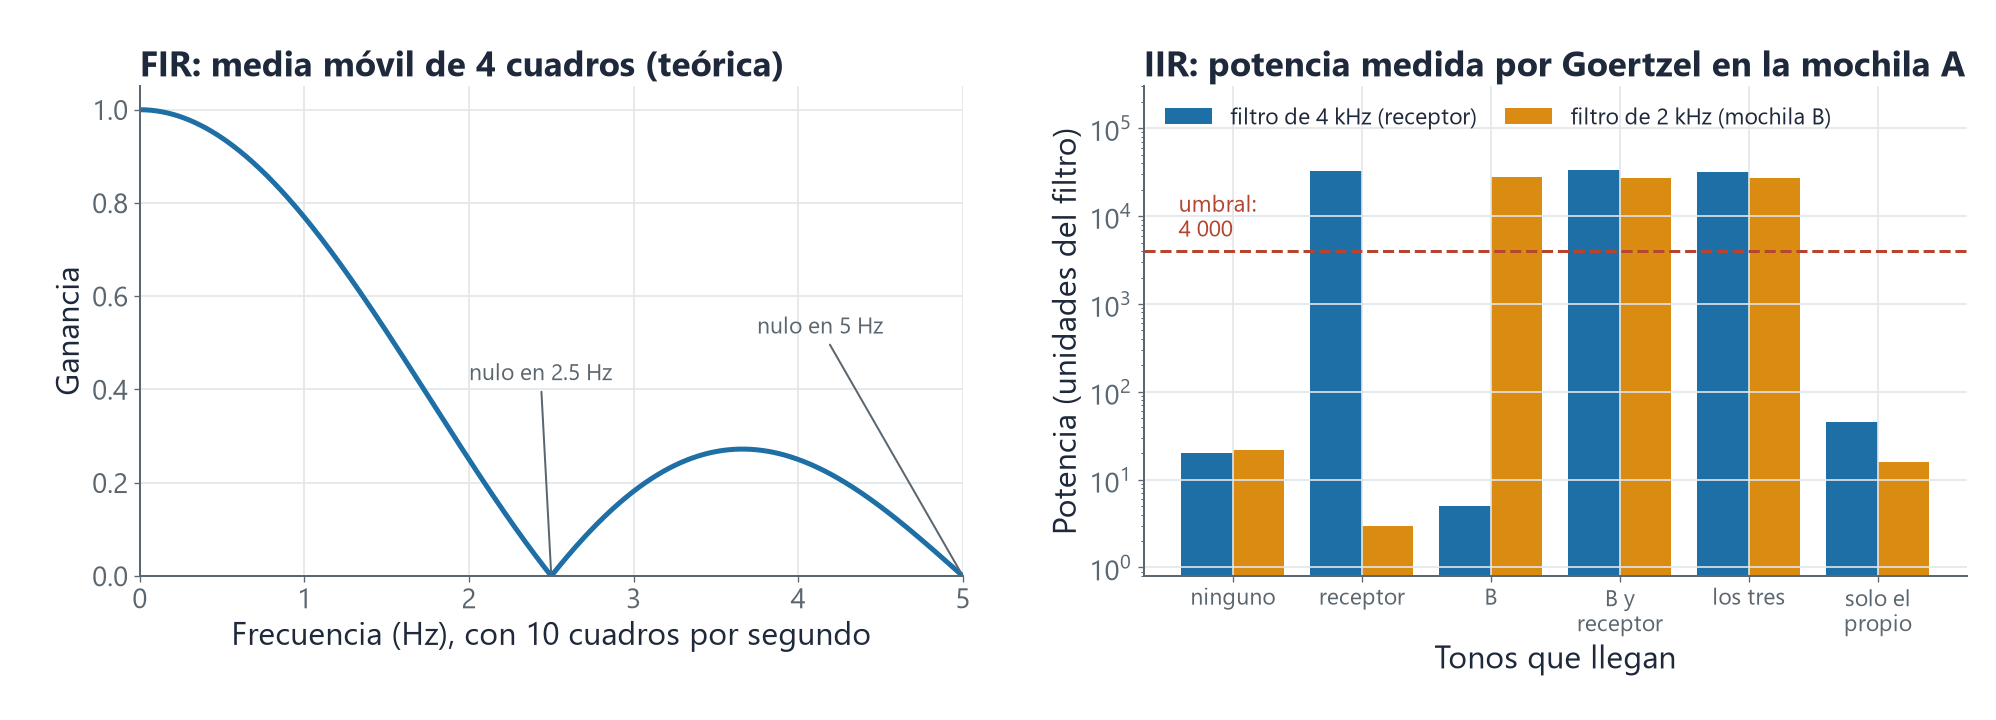
\includegraphics[width=\columnwidth]{filtros.png}
\caption{Izquierda: respuesta de la media móvil. Derecha: potencia medida por los filtros de Goertzel de la mochila A según
los tonos que llegan.}
\label{fig:filtros}
\end{figure}

\textit{PID.} Un controlador posicional en punto fijo,
\begin{equation}
u[n]=K_p e[n]+K_i\textstyle\sum_{k\le n}e[k]+K_d(e[n]-e[n-1]),
\end{equation}
con ganancias Q8.8 e integrador de 32~bits. Si la salida está saturada y el error empuja hacia el mismo lado, congela el acumulador.
Lo corrimos junto a un PID en aritmética real y nunca se separaron una cuenta completa. Con un escalón que satura el actuador, el
sobrepaso es de 0.2~\%; quitando la protección, la salida se queda en el tope y 400 muestras después sigue ahí (fig.~\ref{fig:pid}). Lo pensamos para el modo de
regreso, que dejamos como trabajo futuro.

\begin{figure}[!tb]
\centering
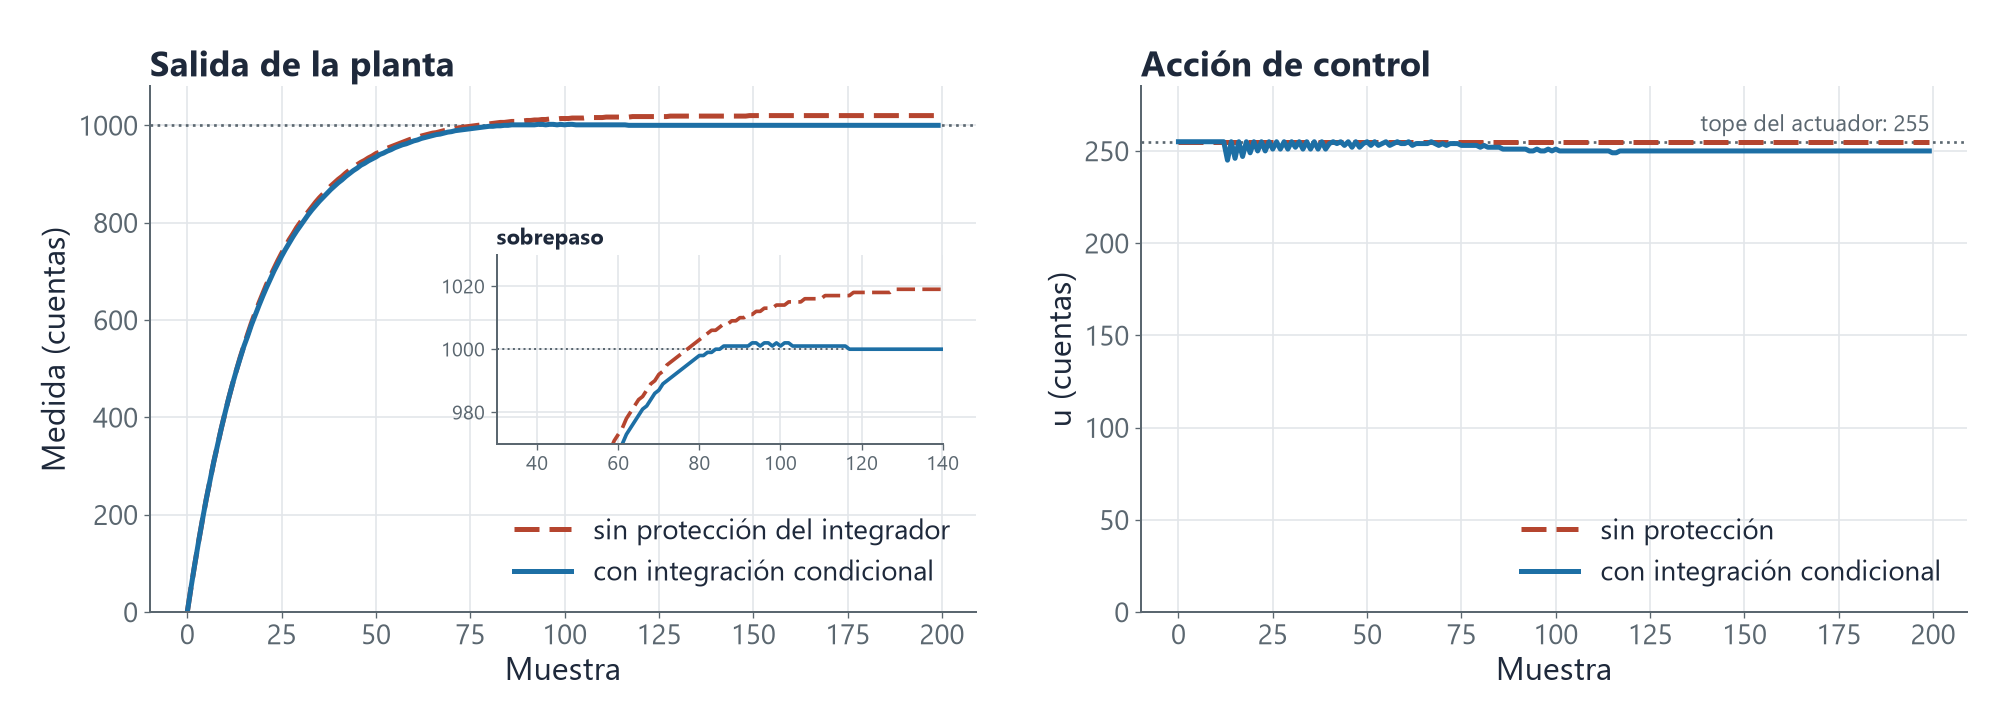
\includegraphics[width=\columnwidth]{pid_respuesta.png}
\caption{PID en punto fijo: escalón de 1\,000 con el actuador saturado, con y sin integración condicional.}
\label{fig:pid}
\end{figure}

\begin{table}[!tb]
\centering\tabfont
\caption{Distancia: CORDIC truncado frente a raíz entera}
\label{tab:dist}
\begin{tabularx}{\columnwidth}{@{}Xrr@{}}
\toprule
Medida & CORDIC & Raíz entera \\
\midrule
Lecturas distintas de la exacta & 17\,762 & 0 \\
Exactas mal leídas, de 4\,179 & 2\,407 & 0 \\
Puntos que contradicen los 32~m & 12 & 0 \\
Elementos lógicos & $\approx500$ & 87--109 \\
Latencia (ciclos) & 18 & 12 \\
\bottomrule
\end{tabularx}
\end{table}

\section{Verificación}

\begin{figure*}[!t]
\centering
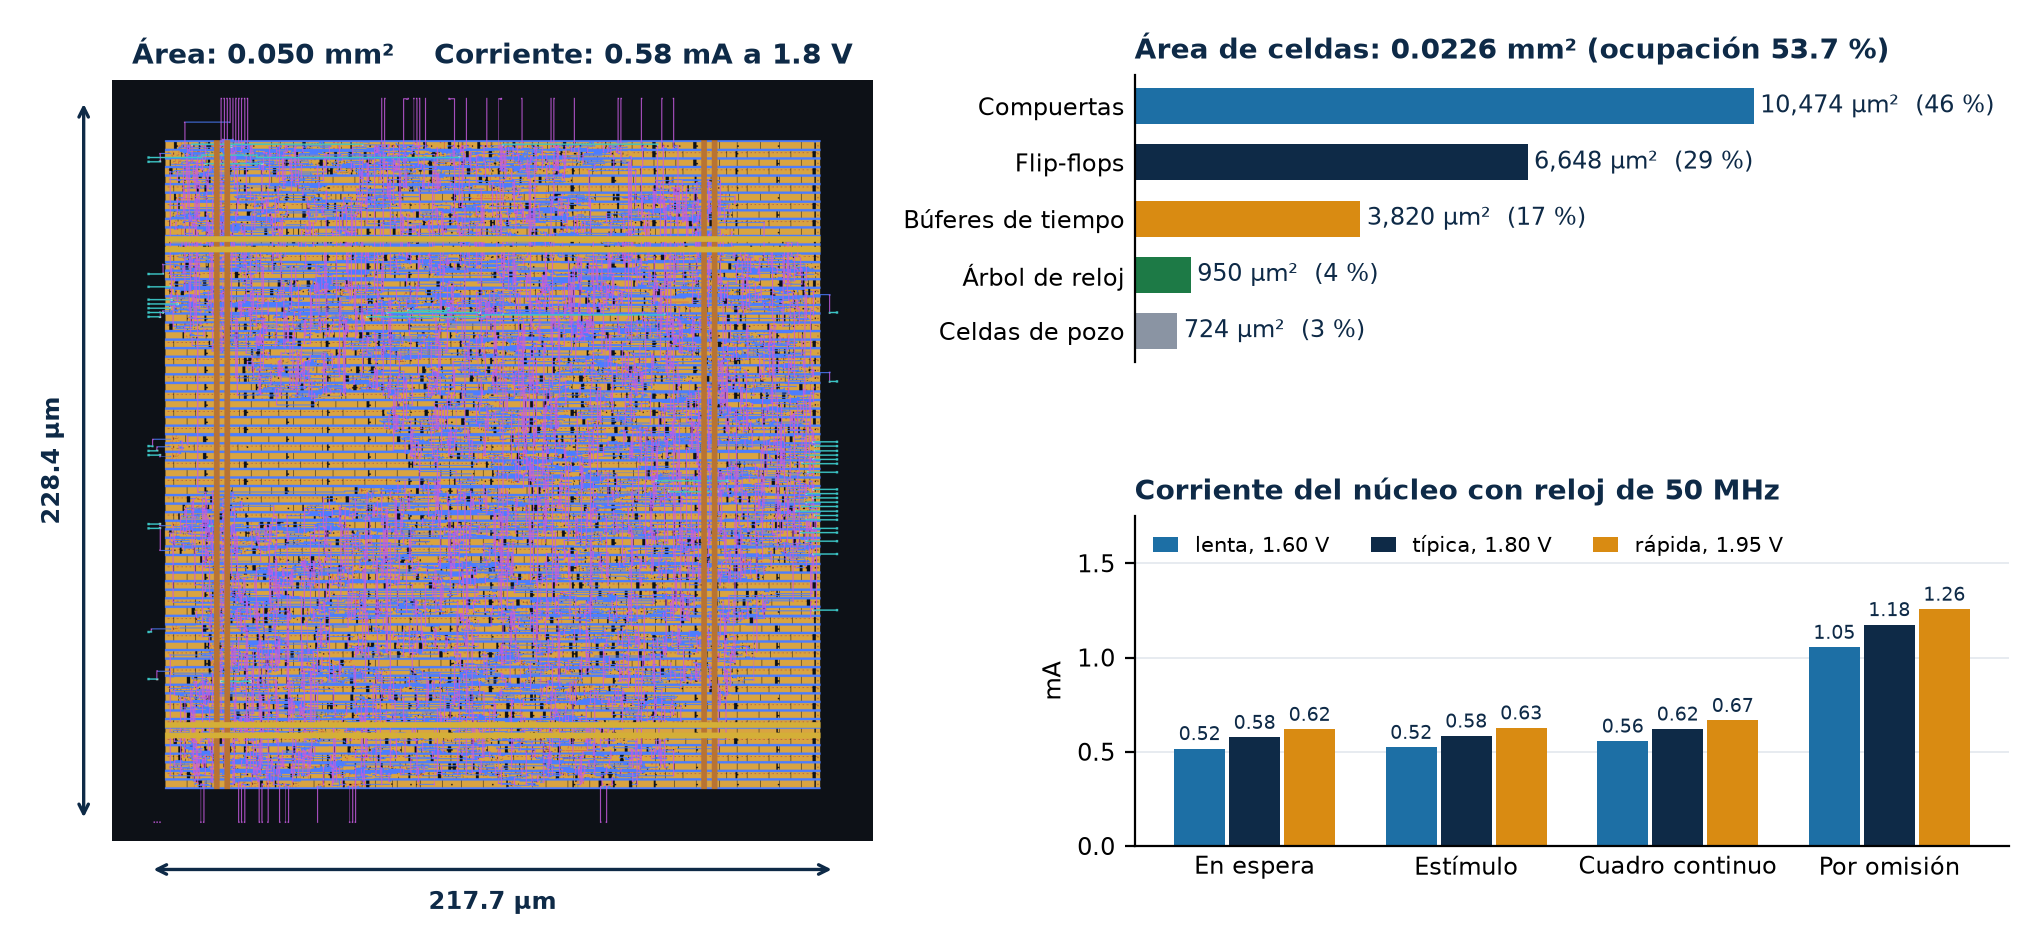
\includegraphics[width=0.90\textwidth]{layout_area_corriente.png}
\caption{Layout del núcleo en SKY130: medidas del dado, reparto del área de celdas y corriente por condición y esquina.}
\label{fig:layout}
\end{figure*}

Verificamos cada bloque por separado antes de conectarlo, con bancos que al final imprimen una línea de resultado
(tabla~\ref{tab:bancos}). El núcleo lo comparamos con un modelo en Python que hace las mismas cuentas enteras, y los bloques numéricos,
con aritmética real. Para la red usamos un banco que conecta las tres FPGA como en el laboratorio y lee displays y LED. La terminal del
operador la probamos contra las tarjetas simuladas con sus módulos superiores.

\begin{table}[!tb]
\centering\tabfont
\caption{Resultados de los bancos de prueba (Icarus Verilog 12)}
\label{tab:bancos}
\begin{tabularx}{\columnwidth}{@{}>{\raggedright\arraybackslash}Xl@{}}
\toprule
Qué se prueba & Resultado \\
\midrule
Núcleo contra modelo de referencia & 11\,424/11\,424 cuadros \\
Sistema por UART hasta la detección & 500/500 respuestas \\
Núcleo e insecto de prueba, una y dos tarjetas & 4/4 y 2/2 \\
CORDIC, divisor & 248/248 \\
Distancia & 89\,443/89\,443 \\
Detector de tonos & 8/8 \\
PID & 3/3 \\
Red de tres FPGA & 9/9 escenarios \\
Terminal del operador & 71/71 \\
\bottomrule
\end{tabularx}
\end{table}

\section{Resultados}

\subsection{Red de tres FPGA}

Los nueve escenarios están en la tabla~\ref{tab:esc}. Con A a 32.00~m (fuera) y B a 31.56~m, el aviso de A llega por B y la persona se
ubica a 6.2~cm de su posición real, 1.10~s después del encendido. También metimos 3~s de pulsos en la línea: se descartaron 16 tramas por
CRC y se contaron 18 perdidas, sin ningún dato equivocado. El corte es exacto. A 31.00~m se oye por ambos ejes y a 32.00~m no; en
diagonal, a 31.96~m sí y a 32.0005~m no (fig.~\ref{fig:umbral}). Al salir de la ventana el conteo baja y al volver sube
(fig.~\ref{fig:seg}).

\begin{table}[!tb]
\centering\tabfont
\caption{Escenarios de la red: 9 de 9 correctos}
\label{tab:esc}
\begin{tabularx}{\columnwidth}{@{}c>{\raggedright\arraybackslash}p{2.0cm}>{\raggedright\arraybackslash}X@{}}
\toprule
N.º & Escenario & Qué se comprobó \\
\midrule
1 & Con puente & A fuera de alcance: conteo 2 en las tres, error de 6.2~cm \\
2 & Bordes & 34, 39 y 47~\textdegree C no; 35 y 38~\textdegree C sí \\
3 & Una mochila & A detecta y B retransmite: conteo 1 en las tres \\
4 & Rumbos opuestos & Se indica y se promedia \\
5 & Botón & Nada caliente: conteo 1 en las tres \\
6 & Sin alcance & Conteo 2, 2 y 0 \\
7 & Sensor & El conteo sigue a la temperatura: 2, 1, 0, 1 \\
8 & Ruido & 16 tramas descartadas, 18 perdidas contadas \\
9 & Corte & 31.00~m sí; 32.00~m no, en los dos ejes \\
\bottomrule
\end{tabularx}
\end{table}

\begin{figure}[!tb]
\centering
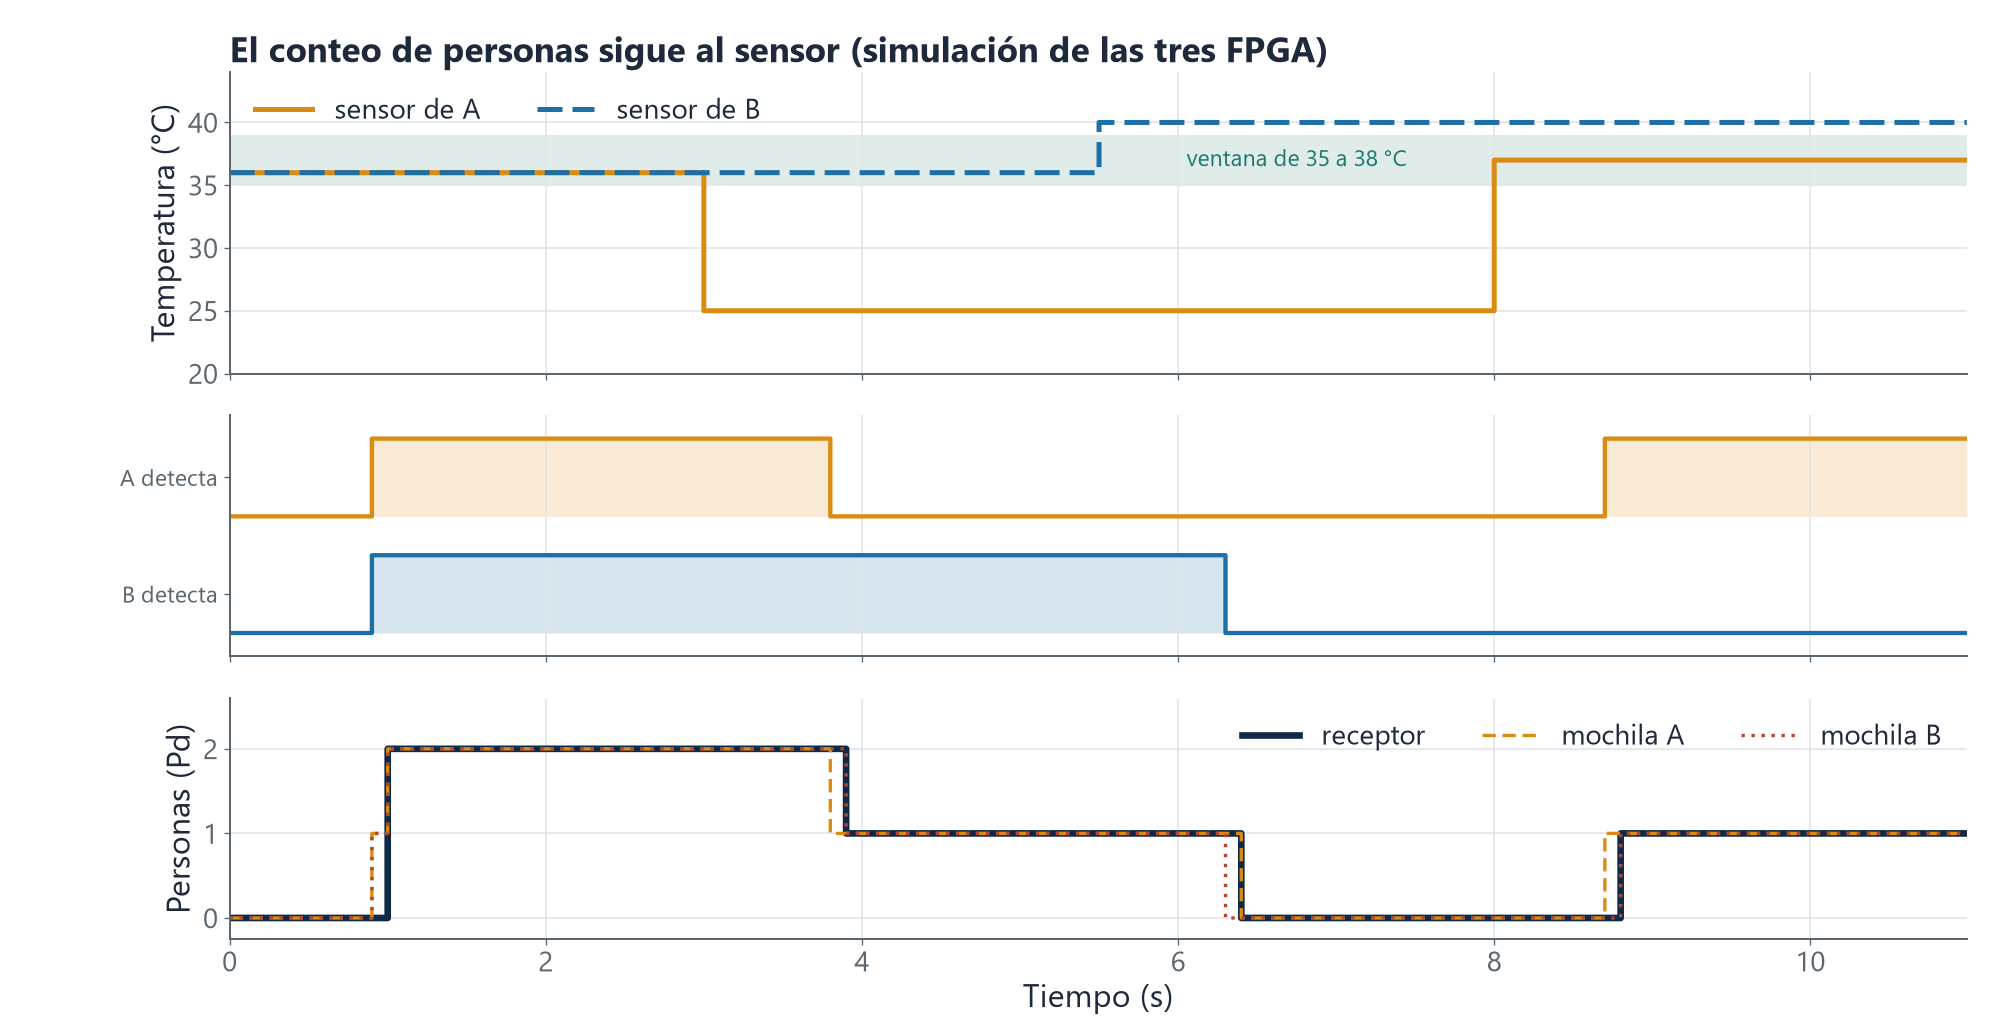
\includegraphics[width=\columnwidth]{red_seguimiento.png}
\caption{Escenario 7: la detección aparece y desaparece unos 0.8~s después del cambio de temperatura; las mochilas
actualizan su conteo un cuadro antes que el receptor.}
\label{fig:seg}
\end{figure}

\begin{figure}[!tb]
\centering
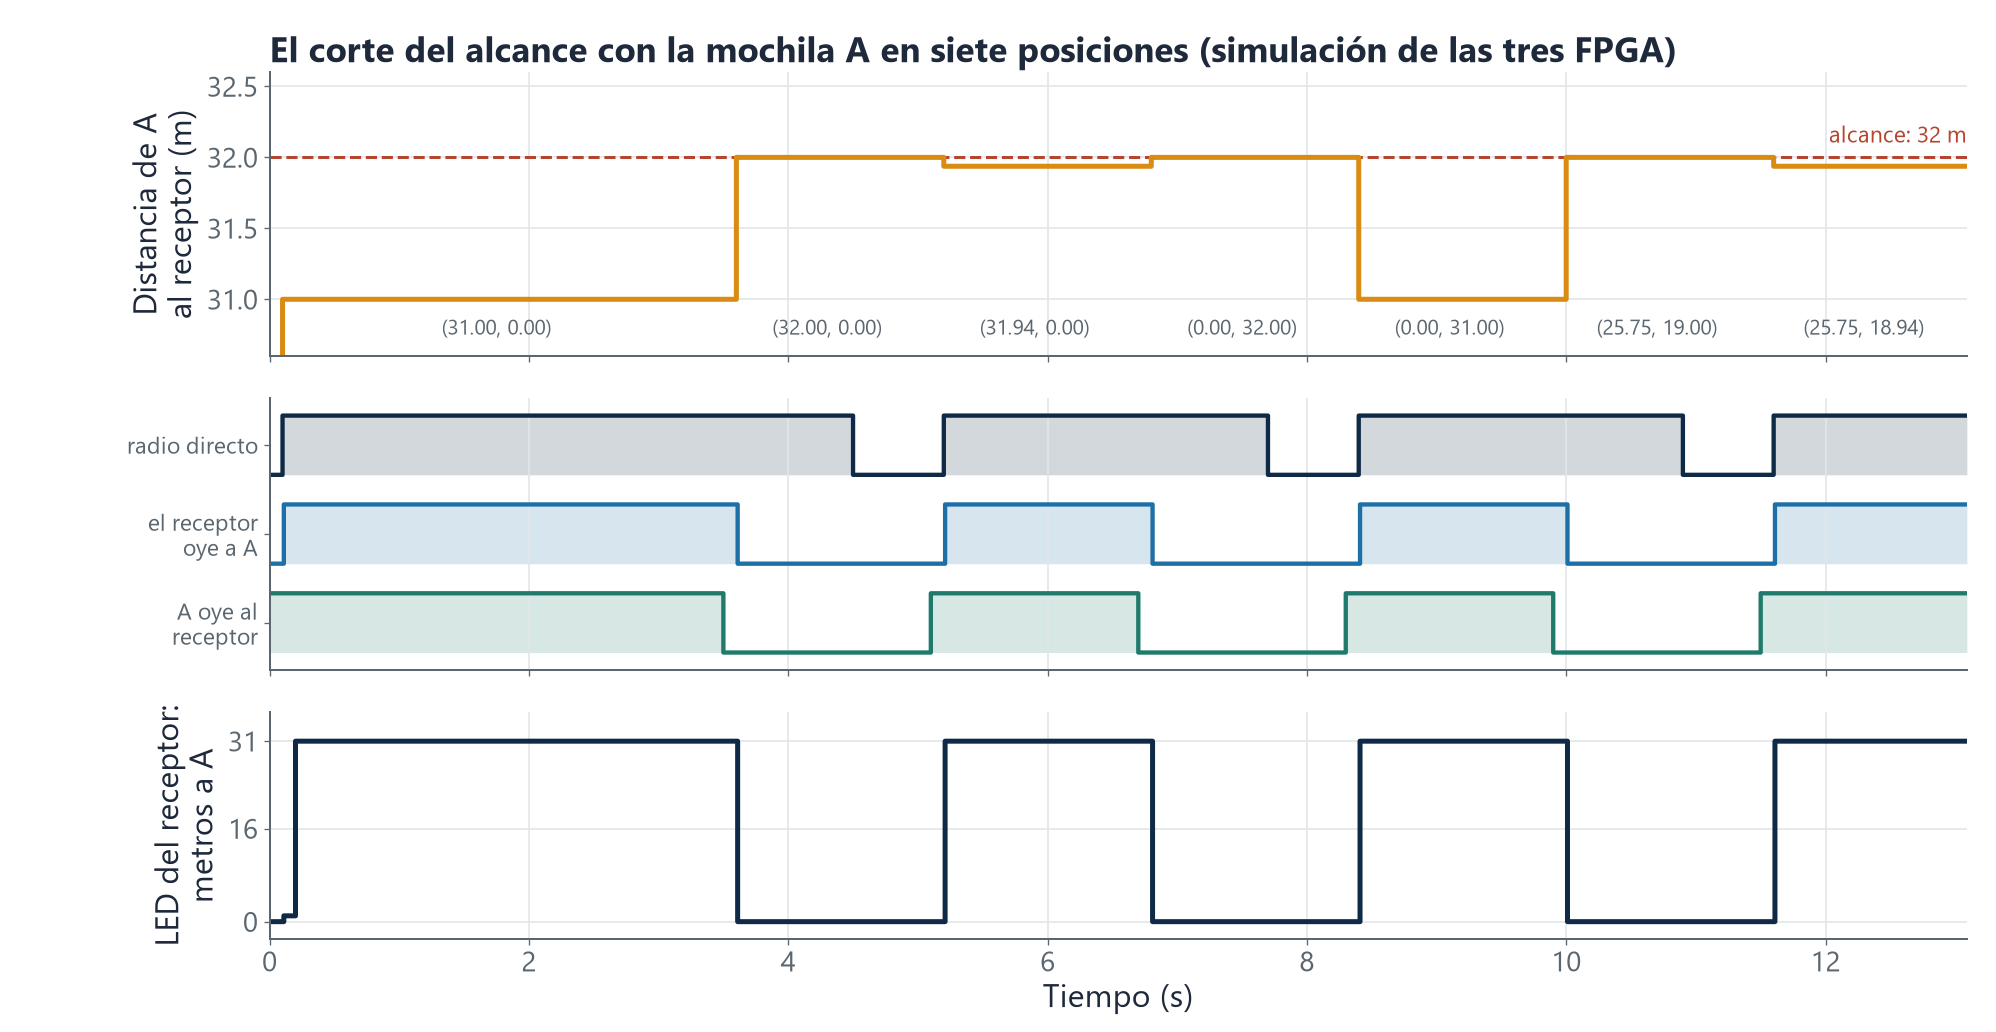
\includegraphics[width=\columnwidth]{red_umbral.png}
\caption{Corte del alcance. Los tonos se pierden al pasar de 32~m; el enlace se da por perdido 1~s después, cuando caduca
la última trama.}
\label{fig:umbral}
\end{figure}

La síntesis está en la tabla~\ref{tab:sint}. En dos tarjetas reales, el núcleo levantó la alerta a los 55.1~s con una persona simulada a
1.65~m (55.6~s en simulación), y no alertó con un objeto a 47.5~\textdegree C, sin persona ni con un insecto que no responde. Con la
versión anterior del enlace corrimos seis escenarios en las tres tarjetas, con 2.8~cm de error en un mapa de 20~m. Después cargamos la
versión que describimos aquí y corrimos los escenarios 1 a 7 y el 9, en varias corridas.

\begin{table}[!tb]
\centering\tabfont
\caption{Síntesis en MAX~10 (10M50DAF484C7G), peor caso, 50~MHz}
\label{tab:sint}
\setlength{\tabcolsep}{4.5pt}
\begin{tabular}{@{}lrrrrr@{}}
\toprule
Variante & EL & Reg. & Mult. & $f_{\max}$ & Holgura \\
 & & & 9~b & (MHz) & (ns) \\
\midrule
Núcleo & 477 & 224 & 0 & 72.08 & 6.13 \\
Mochila A & 3\,933 & 2\,279 & 43 & 55.43 & 1.96 \\
Mochila B & 3\,952 & 2\,279 & 43 & 58.52 & 2.91 \\
Receptor & 4\,929 & 2\,523 & 76 & 61.63 & 3.77 \\
Receptor y B & 7\,525 & 4\,060 & 107 & 59.42 & 3.17 \\
\bottomrule
\end{tabular}\\[2pt]
\raggedright\scriptsize El núcleo se midió dentro del prototipo de 722 elementos lógicos.
\end{table}

\subsection{Layout: área y corriente}

\begin{figure*}[!t]
\centering
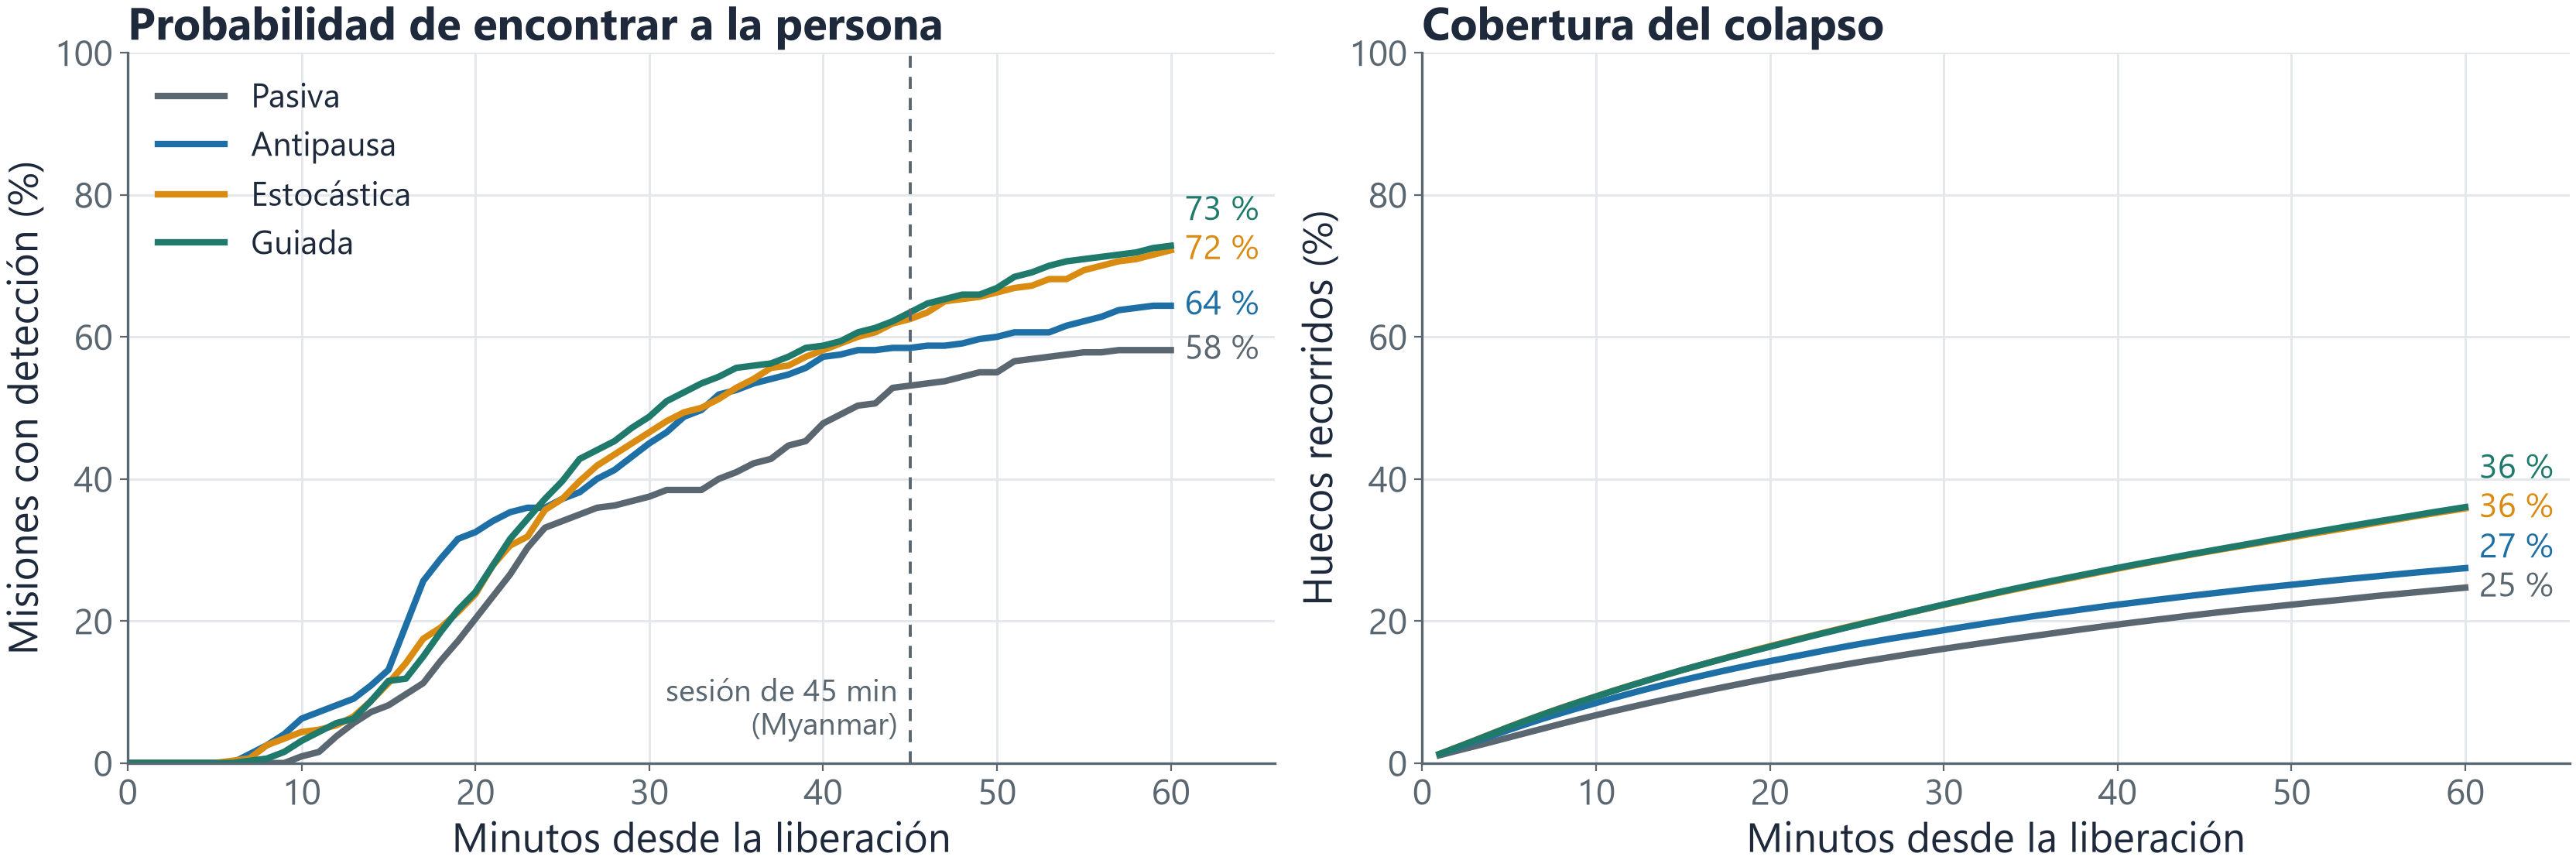
\includegraphics[width=0.455\textwidth]{resultados_politicas.png}\hfill
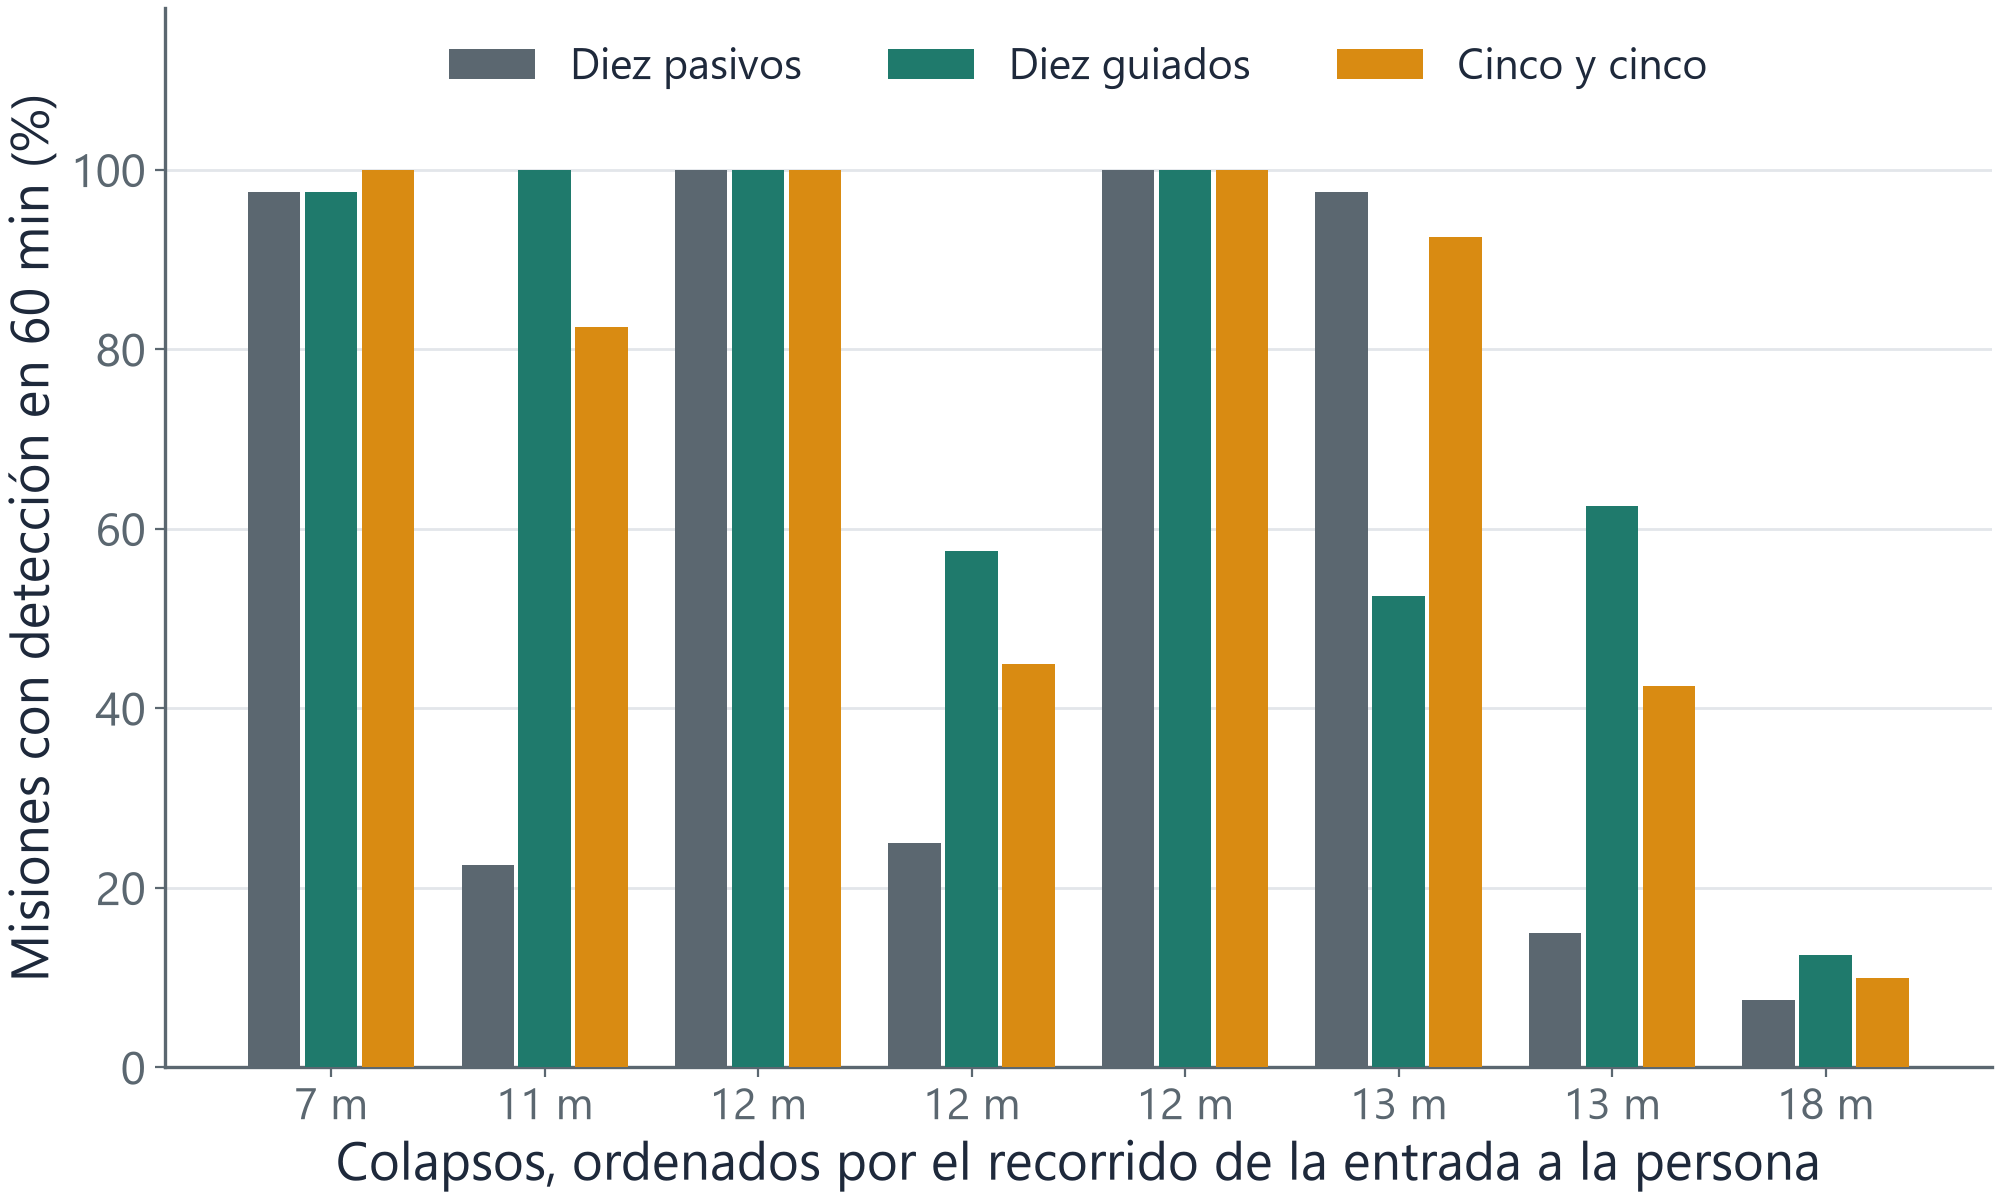
\includegraphics[width=0.275\textwidth]{por_mapa.png}\hfill
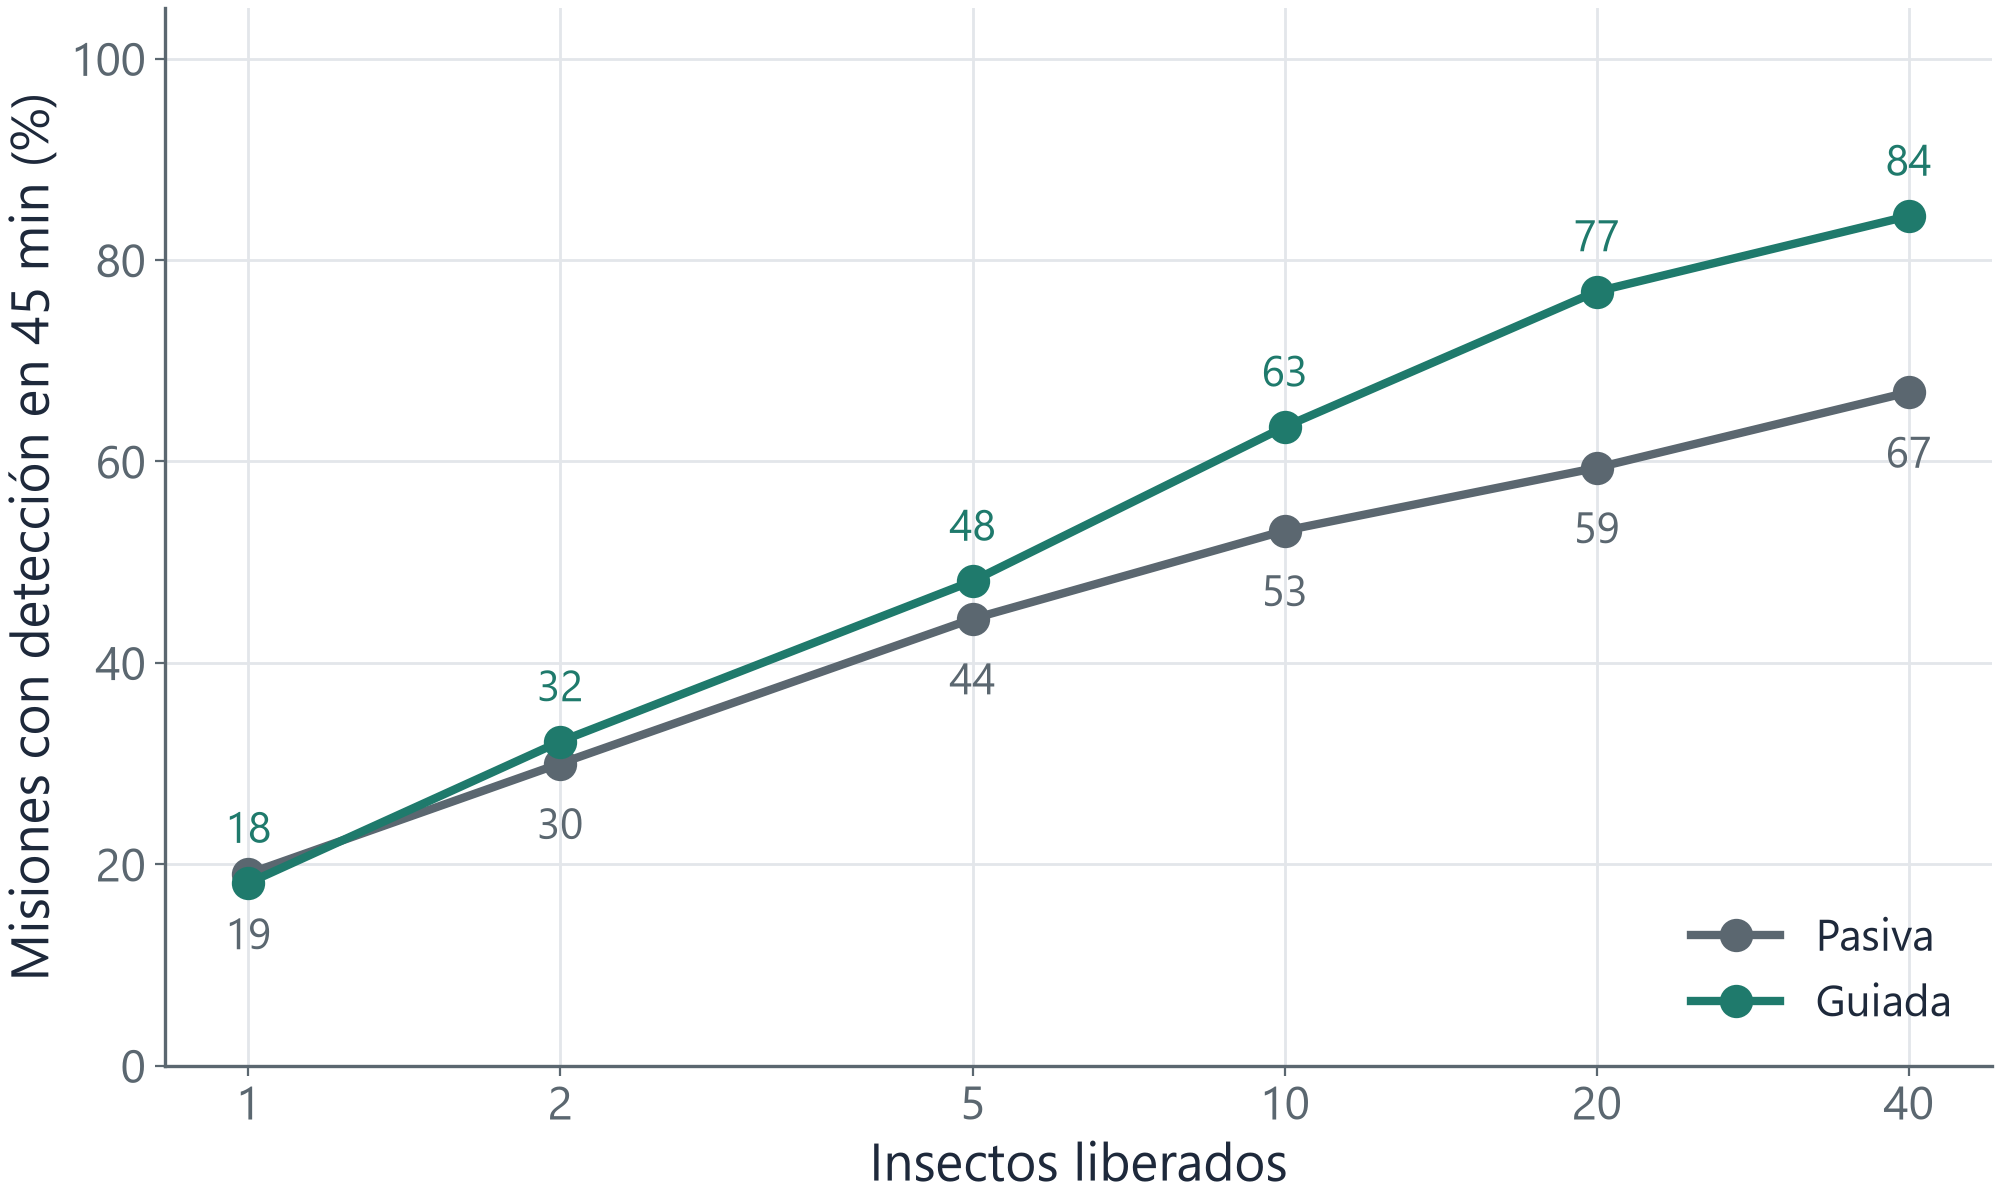
\includegraphics[width=0.25\textwidth]{enjambre.png}
\caption{Misión simulada. Izquierda: detección y cobertura de cuatro políticas con diez insectos. Centro: detección a 60~min
en cada colapso. Derecha: detección a 45~min según el número de insectos.}
\label{fig:pol}
\end{figure*}


Pasamos el núcleo, sin modificarlo, por LibreLane~\cite{librelane}, sucesor de OpenLane~\cite{shalan2020}, con la PDK
\sig{sky130A}~\cite{skywater} y reloj de 20~ns. El GDS no tiene errores de DRC (Magic y KLayout), LVS (Netgen) ni antenas, y cumple
tiempos en las nueve esquinas, con +4.94~ns de \textit{setup} y +0.11~ns de \textit{hold} en la peor. Estimamos una frecuencia de 72~MHz
en la lenta y 143~MHz en la típica. Mide $217.7\times228.4~\mu$m, es decir \textbf{0.050~mm$^2$}, con 0.0226~mm$^2$ de celdas (ocupación
de 53.7~\%), de las que 46~\% son compuertas, 29~\% flip-flops y 17~\% búferes de tiempo (fig.~\ref{fig:layout}).

La corriente la calculamos con OpenSTA sobre el netlist final y los parásitos del ruteo, con la actividad de una simulación de compuertas
(VCD) y, como cota alta, con la actividad por omisión (tabla~\ref{tab:corr}). Casi toda se va en el reloj. En espera, la mitad la gasta su
árbol y la otra mitad los flip-flops que lo reciben. Como el núcleo procesa diez cuadros por segundo, con un reloj de 1~MHz serían unos
12~$\mu$A. Para el mismo prototipo, la FPGA consume 63.5~mA estimados, unas cien veces más que el chip. De todos modos no es donde más se puede ahorrar: de los 30~mW de una mochila (8.1~mA a 3.7~V), al núcleo le toca cerca del 3~\%, y el
sensor y la radio se llevan la mayor parte.

\begin{table}[!tb]
\centering\tabfont
\caption{Corriente del núcleo a 50~MHz (mA)}
\label{tab:corr}
\begin{tabularx}{\columnwidth}{@{}Xrrr@{}}
\toprule
Condición & Lenta & Típica & Rápida \\
 & 1.60~V & 1.80~V & 1.95~V \\
\midrule
En espera & 0.517 & \textbf{0.577} & 0.619 \\
Tren de estímulo & 0.524 & 0.584 & 0.627 \\
Cuadros seguidos & 0.557 & 0.621 & 0.666 \\
Actividad por omisión & 1.054 & 1.175 & 1.257 \\
Potencia en espera (mW) & 0.828 & 1.038 & 1.207 \\
\bottomrule
\end{tabularx}
\end{table}

\subsection{Misión simulada}

Simulamos misiones con agentes en ocho colapsos sintéticos de $8\times6$~m, 320 por caso ($\pm5$ puntos al 95~\%). Para validar, pusimos la marcha junto a la publicada~\cite{dirafzoon2017,tranngoc2024}: cinco de seis medidas coinciden o caen en su
dispersión.
Con diez insectos, la detección en una hora es de 58~\% sin estímulos, 64~\% reactivando al que se detiene, 72~\% con giros al azar y
73~\% guiando hacia el calor (fig.~\ref{fig:pol}), con unos 61 estímulos por insecto y por hora. Con diez guiados se logra lo mismo que con un número de insectos sin guiar entre veinte y cuarenta (68 y 77~\%), el doble o el triple
(fig.~\ref{fig:pol}, derecha). También movimos doce supuestos, uno a la vez, y solo cuatro cambian el resultado más que el margen: el largo del tramo recto (67
a 86~\%), la velocidad que quita la carga (80 a 62~\% si resta 30~\%), la duración de las pausas (86 a 73~\%) y la velocidad de marcha (71
a 81~\%).

El colapso pesa más que la política. La guiada gana en tres de los ocho, empata en cuatro y pierde en uno, donde baja de 98 a 52~\% porque
ahí basta con seguir la pared para llegar a la persona. Un enjambre mixto, cinco y cinco, conserva el promedio (72~\%) y sube ese caso a
92~\%. Con pulsos que habitúan, el presupuesto da la misma detección con la tercera parte de los estímulos (42 frente a 121 por hora), y en eso se ve que dosificar cuida al animal sin costar detecciones. También hay que recoger a los insectos. Un refugio en la entrada recupera 76~\% en
dos horas, y un faro que la mochila siga, 91~\%; guiarlos a ciegas resultó peor (66~\%).

\section{Discusión}

\subsection{Qué decide el desempeño}

La red no tarda 1.10~s por el cálculo, que toma microsegundos, sino por lo que decidimos esperar: la media móvil, los cuatro cuadros de
confirmación y las tramas de 100~ms. Algo que nos dejó este trabajo es que conviene medir contra el valor exacto. Una prueba con tolerancia
de $\pm7$~cm daba por bueno el CORDIC truncado, que fallaba en más de la mitad de las distancias exactas. Del estímulo es de lo que menos datos hay, y por suerte la política no depende mucho de él. Depende bastante más de cuánto y qué tan
rápido camina el insecto, y esa es la razón para mantener ligera la mochila.

\subsection{De la FPGA al chip}

Antes de correr el flujo habíamos estimado 0.014~mm$^2$ por conteo de celdas y nos quedamos cortos, pues se colocaron 0.023~mm$^2$. Los
búferes que cumplen \textit{hold} y transiciones, el árbol de reloj y las celdas de pozo solo aparecen al hacer el layout. El chip tiene 253
flip-flops y la FPGA 224 registros, porque en la tarjeta algunas salidas no se usan y Quartus elimina sus registros. Con los valores por
omisión el flujo pasaba DRC y LVS, pero dejaba 140 transiciones lentas en la esquina lenta; al reparar transiciones después del ruteo
global, con márgenes de 50~\%, quedaron en cero. La alimentación no es problema (cae 0.42~mV, el 0.02~\% de 1.8~V) y frecuencia sobra en las dos tecnologías. Lo que falta mejorar es la
corriente, con un reloj más lento o deteniéndolo entre cuadros.

\subsection{Costo y uso en campo}

Con piezas que se consiguen en tiendas de México, una mochila de prototipo cuesta 1\,031~MXN con la matriz de $8\times8$ y 1\,532~MXN con la
de $32\times24$. Veinte mochilas salen entre 30 y 100 veces más baratas que un binomio canino o un robot de rescate, pero no se pueden comparar así nada
más. El perro encuentra personas y el biobot todavía no lo ha hecho en campo, y en ese precio no está la cría, ni los permisos, ni que el
insecto dura poco. Por eso lo imaginamos como apoyo: el perro marca la zona, el rescatista pone un relevo en el boquete y suelta de diez a
veinte insectos, y cualquier alerta se revisa con cámara o perro antes de mover una losa. Si no llega ninguna, eso no descarta que haya
alguien.

\subsection{Limitaciones y ética}

Al trabajo le faltan varias cosas. El sensor y el canal acústico están simulados en la FPGA y damos por conocida la posición de cada
mochila; el radio es un cable y el alcance, un parámetro. No hicimos pruebas con insectos. La detección falla por encima de unos
30~\textdegree C de ambiente, y la ley mexicana exige mantener a la especie en confinamiento~\cite{lgvs}. Para un despliegue haría falta una autorización que hoy no
existe. Sobre el bienestar del animal no hay consenso~\cite{gibbons2022,adamo2016} y preferimos ser precavidos:
el protocolo que proponemos evita la cirugía, limita la carga a 3~g y los estímulos a 12 acumulados, y pide declarar bajas y destino. Solo se
usarían machos, con doble contención y conteo de entrada y salida. Además hay que recuperar cada mochila, porque su batería es un residuo de
manejo especial.

\section{Conclusiones}

Logramos un núcleo que funciona y cabe en un chip, con 477 elementos lógicos, o 0.050~mm$^2$ y 0.58~mA en SKY130. Con tres FPGA se puede
detectar, avisar y ubicar sin computadora, con 6.2~cm de error a 31.95~m, y la red resiste el ruido y corta exactamente en 32~m. Guiar al
insecto ayuda, pero no siempre, porque depende del colapso; por eso recomendamos el enjambre mixto. Lo que sigue es conectar una matriz
térmica y un micrófono reales, estimar la distancia por tonos, bajar el reloj del núcleo, enviar el GDS a una corrida
compartida~\cite{tinytapeout} y probar en un recinto cerrado con la colonia de la universidad.

El Verilog, los bancos, los proyectos, el layout y los programas de cada figura están en
\url{https://github.com/AdamPark7014/biobot-rescue-proyecto-final}.

\FloatBarrier
\balance
\begin{thebibliography}{99}
\footnotesize
\bibitem{kawata} Y. Kawata, «The Great Hanshin-Awaji Earthquake Disaster», \textit{J. Natural Disaster Science}, vol.~17, n.º~2, 1995. Las proporciones por día provienen de un trabajo del mismo autor de 1996, consultado a través de una cita secundaria.
\bibitem{noji} E. K. Noji, «Public health consequences of earthquakes», Supercourse, Universidad de Pittsburgh. [En línea]. Disponible: \url{https://sites.pitt.edu/~super1/lecture/lec13051/013.htm}
\bibitem{galvis2020} F. Galvis, E. Miranda, P. Heresi, H. Dávalos y J. Ruiz-García, «Overview of collapsed buildings in Mexico City after the 19 September 2017 (Mw7.1) earthquake», \textit{Earthquake Spectra}, 2020, doi: 10.1177/8755293020936694.
\bibitem{murphy2004} R. R. Murphy, «Trial by fire: activities of the rescue robots at the World Trade Center», \textit{IEEE Robot. Autom. Mag.}, vol.~11, n.º~3, pp.~50--61, 2004.
\bibitem{murphy2021} R. R. Murphy, «An expert on search and rescue robots explains the technologies used in disasters like the Florida condo collapse», \textit{The Conversation}, 2021.
\bibitem{tranngoc2023} P. T. Tran-Ngoc \textit{et al.}, «Intelligent insect--computer hybrid robot: installing innate obstacle negotiation and onboard human detection onto cyborg insect», \textit{Adv. Intell. Syst.}, vol.~5, n.º~5, 2200319, 2023.
\bibitem{lin2025} Q. Lin \textit{et al.}, «Cyborg insect factory: automatic assembly for insect-computer hybrid robot via vision-guided robotic arm manipulation of custom bipolar electrodes», \textit{Nat. Commun.}, vol.~16, 6073, 2025.
\bibitem{refat2025} C. M. M. Refat, M. Ariyanto, R. Tanaka, K. Yamamoto y K. Morishima, «Autonomous navigation of bio-intelligent cyborg insect based on insect visual perception», \textit{Adv. Intell. Syst.}, vol.~7, n.º~10, 2400838, 2025.
\bibitem{htx2025} Public Service Division, Gobierno de Singapur, «From lab to rubble», 12 ago. 2026; y «Singapore's cyborg cockroaches helping with search and rescue efforts in Myanmar quake», \textit{The Straits Times}, 5 abr. 2025.
\bibitem{latif2012} T. Latif y A. Bozkurt, «Line following terrestrial insect biobots», en \textit{Proc. IEEE EMBC}, 2012, pp.~972--975.
\bibitem{erickson2015} J. C. Erickson, M. Herrera, M. Bustamante, A. Shingiro y T. Bowen, «Effective stimulus parameters for directed locomotion in Madagascar hissing cockroach biobot», \textit{PLoS ONE}, vol.~10, n.º~8, e0134348, 2015.
\bibitem{sanchez2015} C. J. Sanchez, C.-W. Chiu, Y. Zhou, J. M. González, S. B. Vinson y H. Liang, «Locomotion control of hybrid cockroach robots», \textit{J. R. Soc. Interface}, vol.~12, 20141363, 2015.
\bibitem{ma2023} S. Ma, Y. Chen, S. Yang, S. Liu, L. Tang, B. Li y Y. Li, «The autonomous pipeline navigation of a cockroach bio-robot with enhanced walking stimuli», \textit{Cyborg Bionic Syst.}, vol.~4, 0067, 2023.
\bibitem{lin2023} Q. Lin \textit{et al.}, «Resilient conductive membrane synthesized by in-situ polymerisation for wearable non-invasive electronics on moving appendages of cyborg insect», \textit{npj Flex. Electron.}, vol.~7, 42, 2023.
\bibitem{bai2025} Y. Bai \textit{et al.}, «Swarm navigation of cyborg-insects in unknown obstructed soft terrain», \textit{Nat. Commun.}, vol.~16, 221, 2025.
\bibitem{gracidas2026} E. Gracidas-Reyes, G. Diaz-Arango, H. Vazquez-Leal y F. Marroquin-Gutierrez, «Temperature-dependent tethered locomotion behavior in the Madagascar hissing cockroach using a controlled-environment treadmill platform with exploratory illumination assays», \textit{Biology}, vol.~15, n.º~12, 947, 2026.
\bibitem{montagut2024} M. J. Montagut Marques \textit{et al.}, «Cyborg insect repeatable self-righting locomotion assistance using bio-inspired 3D printed artificial limb», \textit{npj Robot.}, vol.~2, 3, 2024.
\bibitem{dirafzoon2017} A. Dirafzoon, T. Latif, F. Gong, M. Sichitiu, A. Bozkurt y E. Lobaton, «Biobotic motion and behavior analysis in response to directional neurostimulation», en \textit{Proc. IEEE ICASSP}, 2017, pp.~2457--2461.
\bibitem{tranngoc2024} P. T. Tran-Ngoc, H. D. Nguyen, D. L. Le, R. Li, B. S. Chong y H. Sato, «Gait-adaptive navigation and human searching in field with cyborg insect», arXiv:2406.03713, 2024.
\bibitem{peterson1961} W. W. Peterson y D. T. Brown, «Cyclic codes for error detection», \textit{Proc. IRE}, vol.~49, n.º~1, pp.~228--235, 1961.
\bibitem{goertzel1958} G. Goertzel, «An algorithm for the evaluation of finite trigonometric series», \textit{Amer. Math. Monthly}, vol.~65, n.º~1, pp.~34--35, 1958.
\bibitem{volder1959} J. E. Volder, «The CORDIC trigonometric computing technique», \textit{IRE Trans. Electron. Comput.}, vol.~EC-8, n.º~3, pp.~330--334, 1959.
\bibitem{andraka1998} R. Andraka, «A survey of CORDIC algorithms for FPGA based computers», en \textit{Proc. ACM/SIGDA Int. Symp. Field Programmable Gate Arrays}, 1998, pp.~191--200.
\bibitem{librelane} FOSSi Foundation, «LibreLane». [En línea]. Disponible: \url{https://github.com/librelane/librelane} (consultado el 21 nov. 2026).
\bibitem{shalan2020} M. Shalan y T. Edwards, «Building OpenLANE: a 130nm OpenROAD-based tapeout-proven flow», en \textit{Proc. IEEE/ACM Int. Conf. Computer-Aided Design (ICCAD)}, 2020, pp.~1--6.
\bibitem{skywater} SkyWater Technology y Google, «SKY130 process design kit», biblioteca \texttt{sky130\_fd\_sc\_hd}. [En línea]. Disponible: \url{https://github.com/google/skywater-pdk}
\bibitem{lgvs} «Ley General de Vida Silvestre», última reforma publicada en el \textit{Diario Oficial de la Federación} el 16 jul. 2025.
\bibitem{gibbons2022} M. Gibbons, A. Crump, M. Barrett, S. Sarlak, J. Birch y L. Chittka, «Can insects feel pain? A review of the neural and behavioural evidence», \textit{Adv. Insect Physiol.}, pp.~155--229, 2022.
\bibitem{adamo2016} S. A. Adamo, «Do insects feel pain? A question at the intersection of animal behaviour, philosophy and robotics», \textit{Anim. Behav.}, vol.~118, pp.~75--79, 2016.
\bibitem{tinytapeout} Tiny Tapeout. [En línea]. Disponible: \url{https://tinytapeout.com} (consultado el 9 nov. 2026).
\end{thebibliography}


\end{document}
